% !TeX root = ../../libro.tex
% !TeX encoding = utf8

% TODO -- Lista de TODO's:
%
% - [ ] Añadir la fecha de busqueda realizada en SCOPUS
% - [ ] Mover las bases de datos a materiales y métodos
% - [ ] Escribir la sección de motivación
% - [ ] Mover las métricas al comienzo de la parte experimental
% - [ ] ? Quitar secciones en la parte del estado del arte, hacerlo todo en conjunto. Quitar seccion de conclusiones en el estado del arte
% - [ ] ? Formateo de las citas

\chapter{Introducción} \label{ich:introduccion}

Las \textbf{ideas principales} de este trabajo son dos. En primer lugar, resolver un problema de \textbf{reconocimiento facial invariante a cambios en la edad}, por sus siglas en inglés, \entrecomillado{AIFR}. Dentro de este problema, nos centraremos en resolver una tarea de \textbf{retrieval}. En segundo lugar, introducir una nueva técnica de aprendizaje automático, que busca \textbf{solucionar los principales problemas que plantea el uso de la función de pérdida \entrecomillado{triplet loss}} \cite{informatica:principal}. Introduce una forma de generar los \textit{batches} de triples de forma \textit{online}. Evitando así tener un paso separado en el ciclo de entrenamiento, dedicado únicamente a volver a generar de forma \textit{offline} nuevos \textit{batches} de triples. Y de paso, se consigue normalizar la dificultad que suponen estos conjuntos de triples.

Esta situación plantea una serie de \textbf{problemas}:

\begin{itemize}
    \item La nueva técnica de aprendizaje automático se plantea en un \textbf{ambiente completamente distinto} al de \textit{AIFR}, en concreto, en el ámbito de re-identificación de personas.
        \begin{itemize}
            \item En este último, se trabaja normalmente con imágenes de cuerpo completo, y momentos del tiempo muy cercanos. Los problemas que aquí se buscan tratar son, entre otros, seguir identificando con la misma identidad a una persona que ha desaparecido momentáneamente de la escena. Mientras que los problemas principales en \textit{AIFR} son otros (y se detallarán en \customref{ich:descrp_problema})
            \todo{Encontrar un paper que hable de los problemas que tiene re-id. Mirar las introducciones en busca de esto}
            \item Por tanto, no disponemos de literatura en la que se expongan resultados obtenidos de aplicar estas técnicas a nuestro ámbito de trabajo
        \end{itemize}
    \item Esta técnica cambia fundamentalmente la forma de generar \textit{batches} de datos. Y por tanto, modifica en esencia muchas partes primarias del proceso de aprendizaje. Por ejemplo, el ciclo de entrenamiento, el cálculo de métricas durante el entrenamiento, el acceso a los datos. Es por este motivo que hemos tenido que realizar \textbf{implementaciones personalizadas de casi todos estos elementos}, sin poder hacer uso de la mayoría de implementaciones que ofrecen las librerías de aprendizaje automático. Esto supone un \textbf{consumo de tiempo mayor}, teniendo en cuenta que hay que prestar \textbf{especial atención a la optimización y validación} mediante \textit{tests} de estos nuevos módulos
    \item Como comentaremos en \customref{ich:conclusiones}, este trabajo \textbf{no ha dado buenos resultados en la práctica}, comparado con otras técnicas más establecidas en el ámbito del \textit{AIFR}. Sin literatura que aplique nuestras nuevas técnicas en nuestro ámbito, como veremos en \customref{isec:interesareaestudio}, tenemos que \textbf{basarnos en todo el trabajo realizado para estudiar el por qué} de este mal comportamiento.
\end{itemize}

Por otro lado, el ámbito de aplicación de un modelo capaz de reconocer caras independientemente de cambios de edad es amplio, destacando el ámbito de la informática forense. Es muy interesante disponer de un modelo que reconozca caras de sospechosos que llevan en busca un tiempo, o de personas que han desaparecido hace un tiempo y de la que no se disponen imágenes actuales. También para verificar fotografías en documentos de identidad, como pasaportes \cite{informatica:tecnica_sintesis_aifr}.

Y aunque entraremos en detalle en \customref{ich:implementacion}, todo el desarrollo del código y de la presente memoria se ha relaizado en un repositorio abierto de \textit{Github}, en \url{https://github.com/SergioQuijanoRey/TFG}. Allí se pueden consultar todas las ramas desarrolladas, \textit{pull requests}, \textit{issues} y la integración continua con \textit{Github Actions}.

\section{Descripción del problema} \label{ich:descrp_problema}

Como ya se ha comentado, trabajaremos un problema de reconocimiento facial invariante a la edad (\textit{AIFR}, de sus singlas en inglés \entrecomillado{Age-Invariant Face Recognition}), con la idea principal de introducir una variación sobre la función de pérdida \textit{Triplet Loss} para poder generar \textit{batches} de datos de forma \textit{online}. En esta sección nos centraremos en presentar el problema \textit{AIFR}, la nueva técnica de cómputo de la función de pérdida será explorada en profundidad en \customref{isec:triplet_loss}.

El \textbf{problema de reconocimiento facial invariante a la edad} es el siguiente: dada una imagen de una persona a una cierta edad, ser capaces de discriminar entre imágenes de otras personas y de la persona de la que disponemos la primera imagen, teniendo en cuenta cambios significativos en las edades de las personas que aparecen en las imágenes.

Este problema se puede aún especificar más, en las siguientes tareas:

\begin{itemize}
    \item \textbf{\textit{Retrieval}} o búsqueda: dada una imagen de una persona y una base de datos de imágenes, devolver un número específico de imágenes de la misma persona

        \begin{itemize}
            \item Esta es la tarea que se intenta resolver en el presente trabajo
            \item Un escenario para esta tarea es, por ejemplo, tras la desaparición de una persona, tomar imágenes de distintas bases de datos policiales y estudiar las 100 imágenes con mayor potencial de apuntar a la persona indicada
            \item A la acción de aportar una imagen, una base de datos, y tomar las $N$ imágenes que son más probables de coincidir en la identidad de la persona de la primera imagen, la llamaremos \textbf{consulta} o \textbf{\textit{query}}. A la imagen pasada como parámetro se le llama \textbf{\textit{key}} o llave.
        \end{itemize}

    \item Verificación: dadas dos imágenes, el modelo debe decidir si se trata de la misma persona o no.
        \begin{itemize}
            \item Un escenario es, por ejemplo, comprobar la imagen del pasaporte y la imagen obtenida de las cámaras de los puestos de control de acceso automático
        \end{itemize}

    \item Clasificación: habiendo entrenado sobre un conjunto de individuos prefijado, dada una imagen de entrada, identificar al individuo que aparece en dicha imagen como alguno de aquellos vistos durante el entrenamiento
        \begin{itemize}
            \item Esto fuerza a que solo podamos trabajar con un número prefijado de personas, y no con personas arbitrarias que nunca hayamos visto antes. Esta restricción hace que sea la tarea menos interesante (y quizás, la más sencilla de resolver), y por tanto, es inusual encontrar trabajos que usen técnicas relacionadas con las que más adelante presentado para intentar resolver estos problemas
        \end{itemize}
\end{itemize}

Por lo tanto, realmente nuestra tarea es la de realizar \textit{retrieval} de imágenes faciales invariantes a cambios en la edad. Sin embargo, en adelante, salvo que induzca a confusión, nos referiremos a esta tarea simplemente como \textit{AIFR}, sin especificar que estamos realizando concretamente \textit{retrieval} y no otras de las tareas que ya hemos detallado

Este problema tiene, además de los problemas comunes de la visión por computador, las siguientes \textbf{dificultades específicas} \cite{informatica:challenges_retrieval}:

\begin{itemize}
    \item \textbf{Invarianzas}: en nuestro problema esto es especialmente relevante. Al trabajar con imágenes tomadas en, potencialmente, instantes de tiempo muy variados, las características de la imagen pueden variar considerablemente.
        \begin{itemize}
            \item Pensemos, por ejemplo, en fotografías pasadas que fueron tomadas en blanco y negro, en contraste con fotografías más actuales en color
            \item O problemas más relevantes (pues el anterior es fácil de solventar), como cambios relevantes en características de la cámara con la que se toman las fotografías
        \end{itemize}
    \item \textbf{Distractores}: nuestro modelo se debe centrar en estudiar las caras que aparezcan en la imagen, ignorando otros elementos, como los que puedan aparecer en el fondo de las imágenes
    \item \textbf{Eficiencia}: a la hora de que nuestro modelo reciba una \textit{query}, desconocemos el tamaño de la base de datos sobre la que tenemos que operar. Por tanto, nuestro modelo deberá ser eficiente para poder trabajar con grandes bases de datos sin que el tiempo de respuesta se vea gravemente afectado
    \item Problemas asociados al bold{envejecimiento}: cómo varía la cara con el paso de los años es un proceso muy complejo. Algunos de los factores que afectan a este envejecimiento \cite{informatica:tecnica_sintesis_aifr} son:
        \begin{itemize}
            \item Factores intrínsecos como la genética o la etnia
            \item Factores extrínsecos como el ambiente o los hábitos de vida
        \end{itemize}
    Además, algunas características de la cara cambian drásticamente con el paso de los años. Por ejemplo, la textura (pensar por ejemplo en la aparición de arrugas, lunares, vello, \ldots), cambios en la forma de la cara (por ejemplo, por un cambio en el peso corporal)

\item Tenemos que trabajar con \textbf{identidades que nunca hemos visto} en nuestros datos de entrenamiento. En otras tareas, como por ejemplo la de clasificación de objetos cotidianos, también ocurre esto (por ejemplo, tenemos imágenes de coches que nunca ha visto previamente el modelo). Sin embargo la diferencia radica en que, en nuestro problema, el modelo debe saber identificar identidades, mientras que en el segundo caso, el modelo debe saber identificar categorías. Siguiendo con esta analogía, sería como pedirle al modelo clasificador que, dados dos tipos de objetos que nunca ha visto (por ejemplo, aviones), sepa asignarles la misma categoría

\item Nuestro modelo debe identificar como similares (véase \customref{isec:embeddings}) imágenes de la misma persona, aunque sea en momentos muy distintos. Y debe identificar como no similares imágenes de personas distintas. Es muy fácil que ocurra que la imagen de la misma persona en dos edades alejadas parezca más distinta que las imágenes de dos personas distintas pero de la misma edad. Por ejemplo, esto se puede ver en \customref{img:messi_distintos_otro_adulto}

\item Aunque desarrollemos esto más tarde en \customref{isec:base_datos_usada}, los \textbf{\textit{datasets} de \textit{AIFR} son escasos y presentan problemas} \cite{informatica:tecnica_sintesis_aifr}. Algunas de estas bases de datos son muy pequeñas. Otras, son de un tamaño más grande, pero presentan mucha menos variabilidad en los rangos de edad. Y por supuesto, muchas de estas bases de datos presentan problemas de representatividad (etnia, sexo).
\end{itemize}

\begin{figure}[H]
\centering
    \begin{subfigure}{0.5\textwidth}
        \centering
        \includegraphics[width=0.5\linewidth]{informatica/messi_niño}
        \caption{Edad temprana. Imagen extraída de \cite{informatica:webimg_messi_pequeno}}
        \label{img:messi_pequeno}
    \end{subfigure}%
    \begin{subfigure}{.5\textwidth}
        \centering
        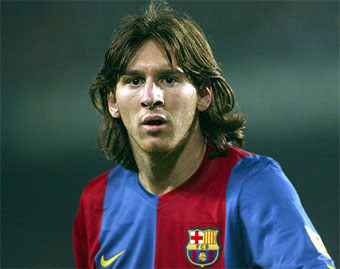
\includegraphics[width=0.8\linewidth]{informatica/messi_joven}
        \caption{Edad joven. Imagen extraída de \cite{informatica:webimg_messi_joven}}
    \end{subfigure}%

    \begin{subfigure}{.5\textwidth}
        \centering
        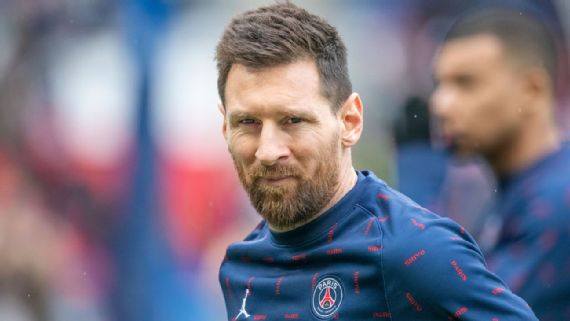
\includegraphics[width=0.6\linewidth]{informatica/messi_adulto}
        \caption{Edad adulta. Imagen extraída de \cite{informatica:webimg_messi_adulto}}
        \label{img:messi_adulto}
    \end{subfigure}%
    \begin{subfigure}{.5\textwidth}
        \centering
        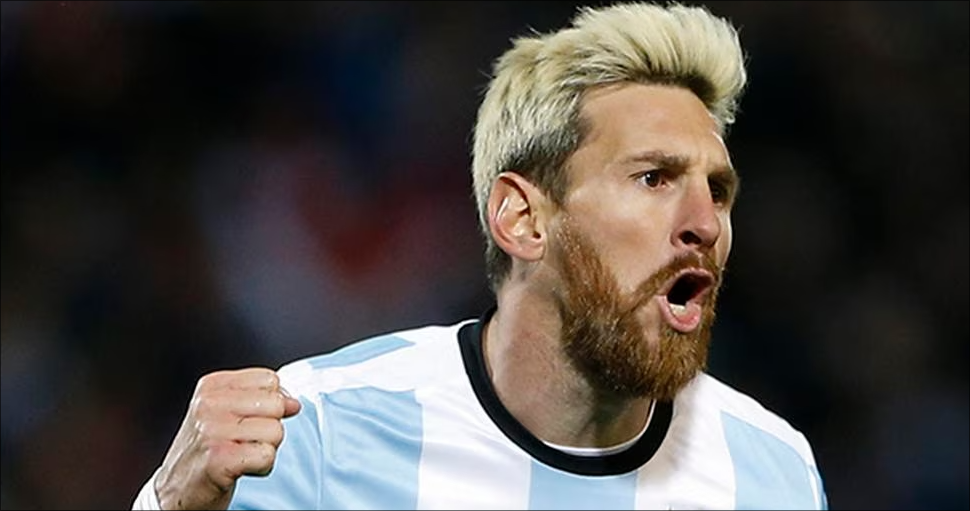
\includegraphics[width=0.8\linewidth]{informatica/messi_rubio}
        \caption{Otra imagen en la edad adulta, pocos años después. Imagen extraída de \cite{informatica:webimg_messi_rubio}}
    \end{subfigure}

    \caption{Lionel Messi en cuatro momentos distintos de su vida}
    \label{img:messi_cuatro_edades}

\end{figure}

Por poner un ejemplo, fijémonos en \customref{img:messi_cuatro_edades}. Estas cuatro imágenes reflejan perfectamente los problemas que hemos planteado previamente. Por ejemplo, en la fotografía \ref{img:messi_adulto} podemos ver que, en el fondo de la imagen, aparece otro jugador, y nuestro modelo podría distraerse por este hecho. La imagen en la que aparece siendo más pequeño, \ref{img:messi_pequeño}, es de una calidad mucho menor que el resto de imágenes. No ha desarrollado todavía rasgos faciales muy característicos. La variabilidad en el estilo de pelo es total. Se puede apreciar perfectamente como el paso de los años va modificando los rasgos de la cara. Y todo esto sin comentar problemas comunes y bien conocidos en la visión por computador, como por ejemplo, cambios en la pose, iluminación, \ldots

Veámos otro ejemplo:

\begin{figure}[H]
\centering
    \begin{subfigure}{0.5\textwidth}
        \centering
        \includegraphics[width=0.6\linewidth]{informatica/messi_niño}
        \caption{Messi en una edad temprana}
    \end{subfigure}%
    \begin{subfigure}{.5\textwidth}
        \centering
        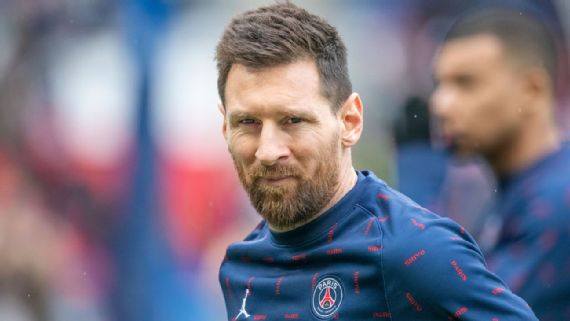
\includegraphics[width=0.8\linewidth]{informatica/messi_adulto}
        \caption{Messi en edad adulta}
    \end{subfigure}

    \begin{subfigure}{.8\textwidth}
        \centering
        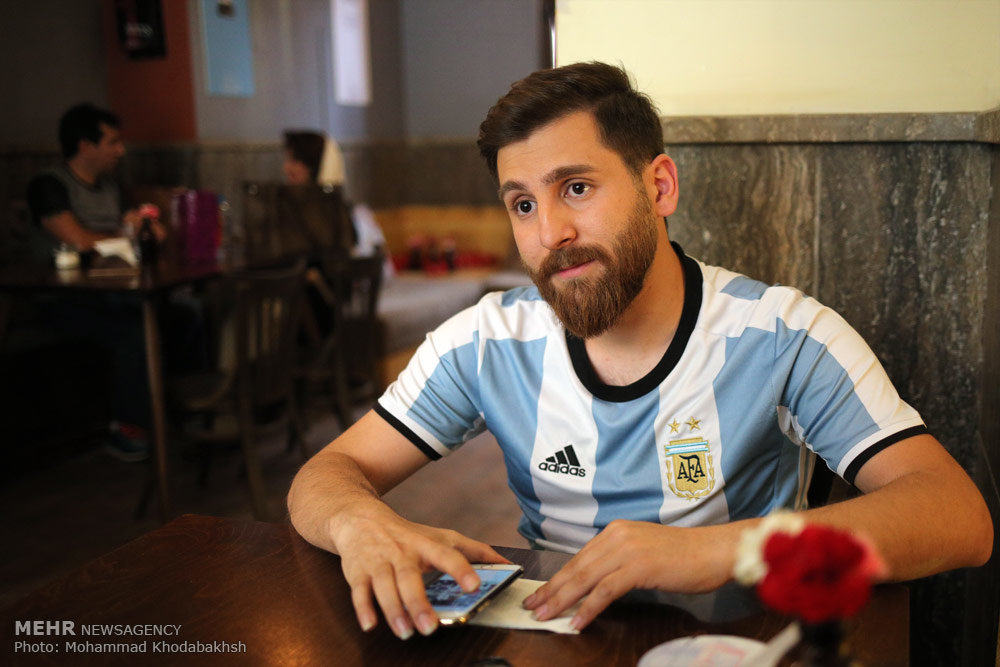
\includegraphics[width=0.6\linewidth]{informatica/doble_messi}
        \caption{Riza Perestes, ciudadano iraní. Imagen extraída de \url{https://www.insideworldsoccer.com/2017/04/riza-perestes-iran-soccer-fan-lionel-messi-lookalike.html?m=0}}
    \end{subfigure}

\caption{Lionel Messi en dos momentos distintos de su vida, y un Riza Perestes, ciudadano iraní con gran parecido}
\label{img:messi_distintos_otro_adulto}
\end{figure}

En este ejemplo vemos un problema que hemos comentado previamente: tenemos más parecido entre dos personas distintas pero de la misma edad, que entre la misma persona pero a distintas edades. En este caso el parecido es extraordinario, pero es razonable que nuestro modelo tenga dificultades en asignar mayor parecido a las dos imágenes de distintas edades, que a la imagen de otro individuo con barba y corte de pelo parecido.

Ahora, aunque más tarde desarrollemos en profundidad el uso de \textit{triplet loss} (\customref{isec:triplet_loss}), conviene hacer ahora unos pequeños apuntes sobre esta técnica. Para empezar, el uso de esta función de pérdida ya nos indica que, de una forma u otra, nuestra solución al problema va a fundamentarse en el cómputo de un \textit{embedding}.

Por tanto, usando dicho fundamento, podríamos haber resuelto también alguno de los otros problemas que ya hemos mencionado, por ejemplo, el de verificación. Sin embargo, para acotar el alcance de este trabajo, hemos decidido centrarnos en \textit{retrieval}.

Además, por cómo hemos diseñado el código (basado en adaptadores, como explicamos en \customref{ich:implementacion}), la adaptación del modelo a una nueva tarea es inmediato, y en teoría, si el modelo inicial es competente, el modelo adaptado también debería serlo.

Y para finalizar, comentaremos los \textbf{dos enfoques principales usados para resolver problemas de \textit{AIFR}}:

\begin{enumerate}
    \item El primer enfoque es aplicar modelos generativos adversarios (\textit{GAN}). Por ejemplo, el \textit{Age Invariant Model} o \textit{AIM} propuesto en \cite{informatica:tecnica_sintesis_aifr}.
    \item El segundo enfoque es directamente trabajar sobre una base de datos que presente la suficiente variabilidad en la edad de los individuos, y desarrollar un modelo que realice nuestra tarea. Este enfoque casi siempre pasa por computar un \textit{embedding}. Este será el enfoque que sigamos.
\end{enumerate}
\todo{\cite{informatica:paper_cacd} habla en la página 3 de \url{http://www.sirius.umiacs.io/papers/chen14tmm.pdf} de las aproximaciones al problema!}

\section{Motivación}

\todo{Desarrollar}


\section{Descripción de las bases de datos usadas} \label{isec:base_datos_usada}

Como se comentará en \customref{isec:planificacion}, teniendo en cuenta que íbamos a tener que realizar un gran número de implementaciones, decidimos iterar sobre varias bases de datos.

\subsection{MNIST}

La \textbf{primera base de datos} que consideramos es la más que conocida \entrecomillado{MNIST} \cite{informatica:mnist}. Esta base de datos se compone de 70000 imágenes $28 \times 28$ de dígitos, del 0 al 9, escritos a mano. No tiene ningún interés para el trabajo que vamos a realizar. Sin embargo, escogemos esta base de datos como punto de partida porque:

\begin{itemize}
    \item Es una base de datos muy pequeña, por lo que nuestras implementaciones no tendrán ningún tipo de problemas de rendimiento
    \item Es una base de datos muy sencilla, no tenemos que preocuparnos de procesar las imágenes de ninguna forma
    \item No tenemos que realizar ninguna implementación para trabajar con ella, puesto que podemos usar el paquete \lstinline{torchvision}, que se encarga de la descarga del conjunto de datos y su disposición en un objeto de tipo \lstinline{torch.utils.data.Dataset}
\end{itemize}

\begin{figure}[H]
    \centering
    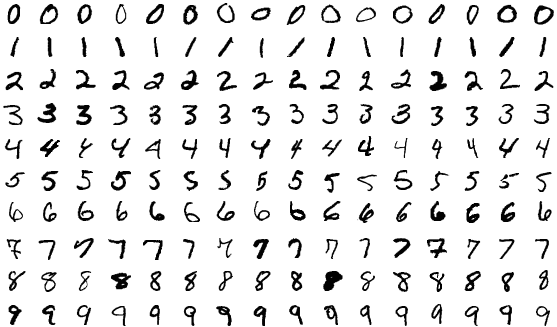
\includegraphics[width=0.5\textwidth]{informatica/ejemplo_mnist}
    \caption{Muestra de ejemplo de los dígitos del \textit{dataset} \textit{MNIST}}
\end{figure}


\subsection{Labeled Faces in the Wild}

La \textbf{segunda base de datos} con la que trabajamos es \textit{Labeled Faces in the Wild} (\textit{LFW}) \cite{informatica:lfw_dataset}. La base de datos se compone de algo más de 13000 imágenes de caras extraídas de la web, en la que aparecen 5749 individuos.

\begin{figure}[H]
    \centering
    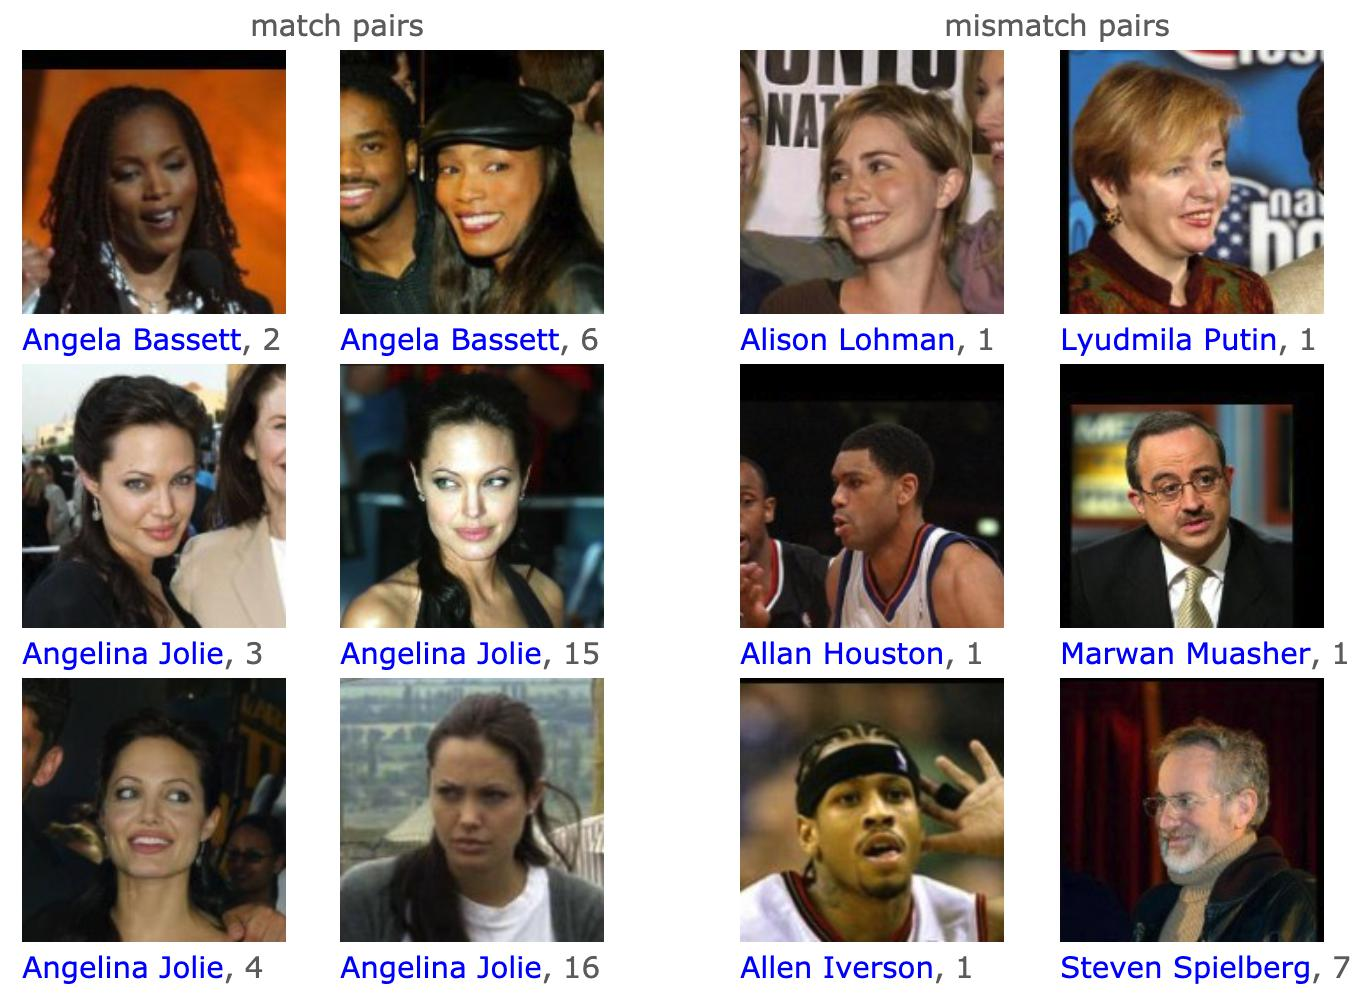
\includegraphics[width=0.5\textwidth]{informatica/ejemplo_lfw}
    \caption{Muestra de ejemplo del \textit{dataset} \textit{LFW}. Imagen extraída de \cite{informatica:papers_with_code_lfw}}
\end{figure}

En este caso damos un salto de calidad en cuanto a lo adecuada que es la base de datos a nuestro problema. Principalmente:

\begin{itemize}
    \item Estamos trabajando con imágenes faciales
    \item El tamaño del \textit{dataset} ha aumentado considerablemente. Como veremos más adelante, en \customref{isec:optimizacion_codigo}, esto ya hace que tengamos que plantearnos optimizaciones de nuestros módulos de código
    \item La tarea de \textit{retrieval} ya tiene sentido (esto no ocurría al trabajar con dígitos manuscritos)
\end{itemize}

Aunque tenemos una serie de \textbf{problemas con esta base de datos}, que motiva el uso de las dos últimas bases de datos:

\begin{itemize}
    \item En primer lugar, y como se indica en \cite{informatica:lfw_dataset}, esta base de datos está pensada para resolver una tarea de verificación. Aunque nos centremos en computar un \textit{embedding} (tarea que deberíamos poder resolver sin problemas), la propia institución ya nos está advirtiendo sobre lo inadecuada de la base de datos
    \item Hay grupos que no están propiamente representados. Por ejemplo, apenas hay niños o personas por encima de los 80 años. Las mujeres y ciertos grupos étnicos están infrarrepresentados. En nuestro caso, es \textbf{especialmente grave la infrarrepresentación de ciertos grupos de edad}
    \item Más tarde introduciremos, en \customref{ich:fundamentos_teoricos}, la función de pérdida \textit{triplet loss} y las técnicas para computarla de forma \textit{online}, usando \textit{P-K sampling}. Para esto, es fundamental que cada individuo tenga el máximo número de fotografías. De nada nos sirve, por ejemplo, tener una base de datos enorme pero con solo una fotografía por persona. En este sentido, y como indica \cite{informatica:lfw_dataset}, solo 1680 individuos tienen dos fotografías o más. Esto hace que tomar valores altos en el \textit{P-K sampling} sea imposible, y que por ello, tengamos que recurrir al aumentado de datos. Como comentaremos en \customref{isec:aumentado_datos}, esto será un reto importante de cara a mantener un rendimiento aceptable
    \item Este \textit{dataset} no introduce ninguna forma de trabajar la invarianza a cambios de edad, por lo que, en última instancia, no es adecuado para nuestros propósitos
\end{itemize}

De hecho, en la siguiente figura podemos observar la distribución del número de imágenes por cada individuo:

\begin{figure}[H]
    \centering
    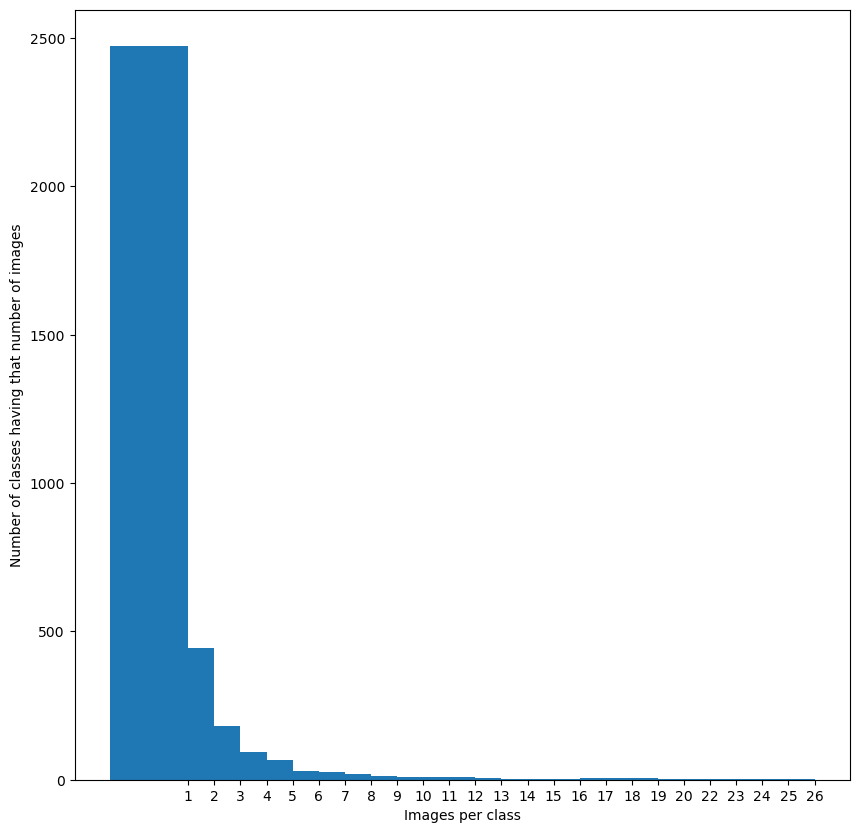
\includegraphics[width=0.6\textwidth]{informatica/lfw_images_per_class}
    \caption{Distribución del número de imágenes por cada individuo. En el eje horizontal, tenemos el número de imágenes por cada individuo. En vertical, la cantidad de individuos que tienen un cierto número de imágenes}
\end{figure}

Podemos ver que la mayoría de individuos solo tienen una imagen o dos. Teniendo en cuenta que casi siempre trabajamos usando al menos tres imágenes por clase, queda clara la necesidad de usar aumento de datos, que introduciremos en \customref{isec:aumentado_datos}. Adelantándonos a lo que presentaremos en el aumento de datos, veámos cómo queda esta distribución tras forzar que cada individuo tenga al menos un número dado de datos:

\begin{figure}[H]
\centering
    \begin{subfigure}{0.5\textwidth}
        \centering
        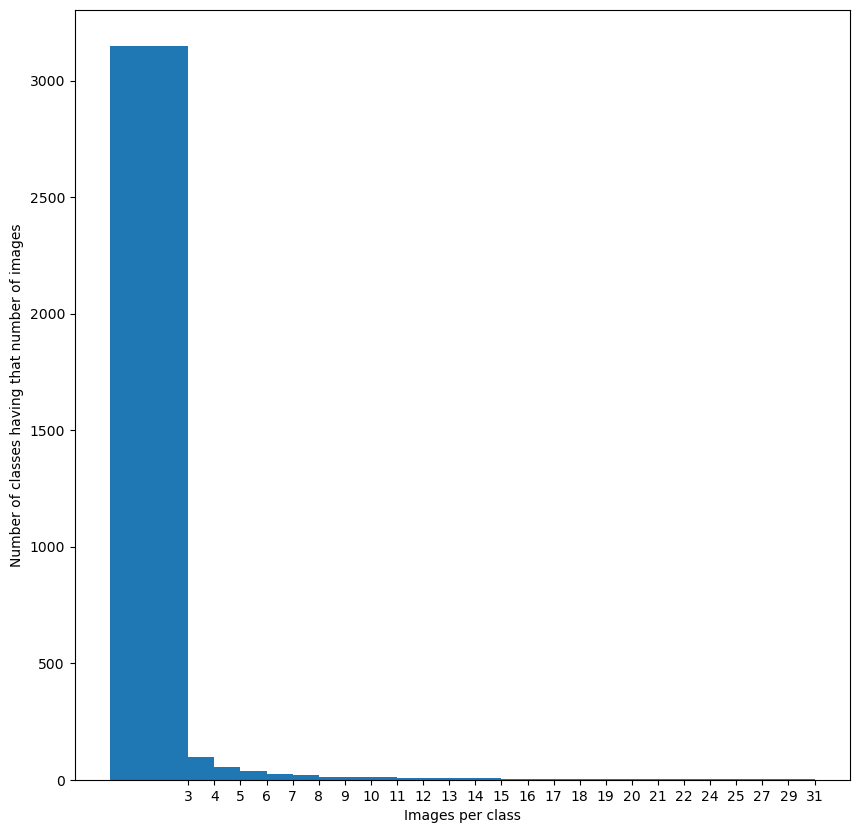
\includegraphics[width=.7\linewidth]{informatica/lfw_forzar_3}
        \caption{Forzando 3 imágenes por individuo }
    \end{subfigure}%
    \begin{subfigure}{.5\textwidth}
        \centering
        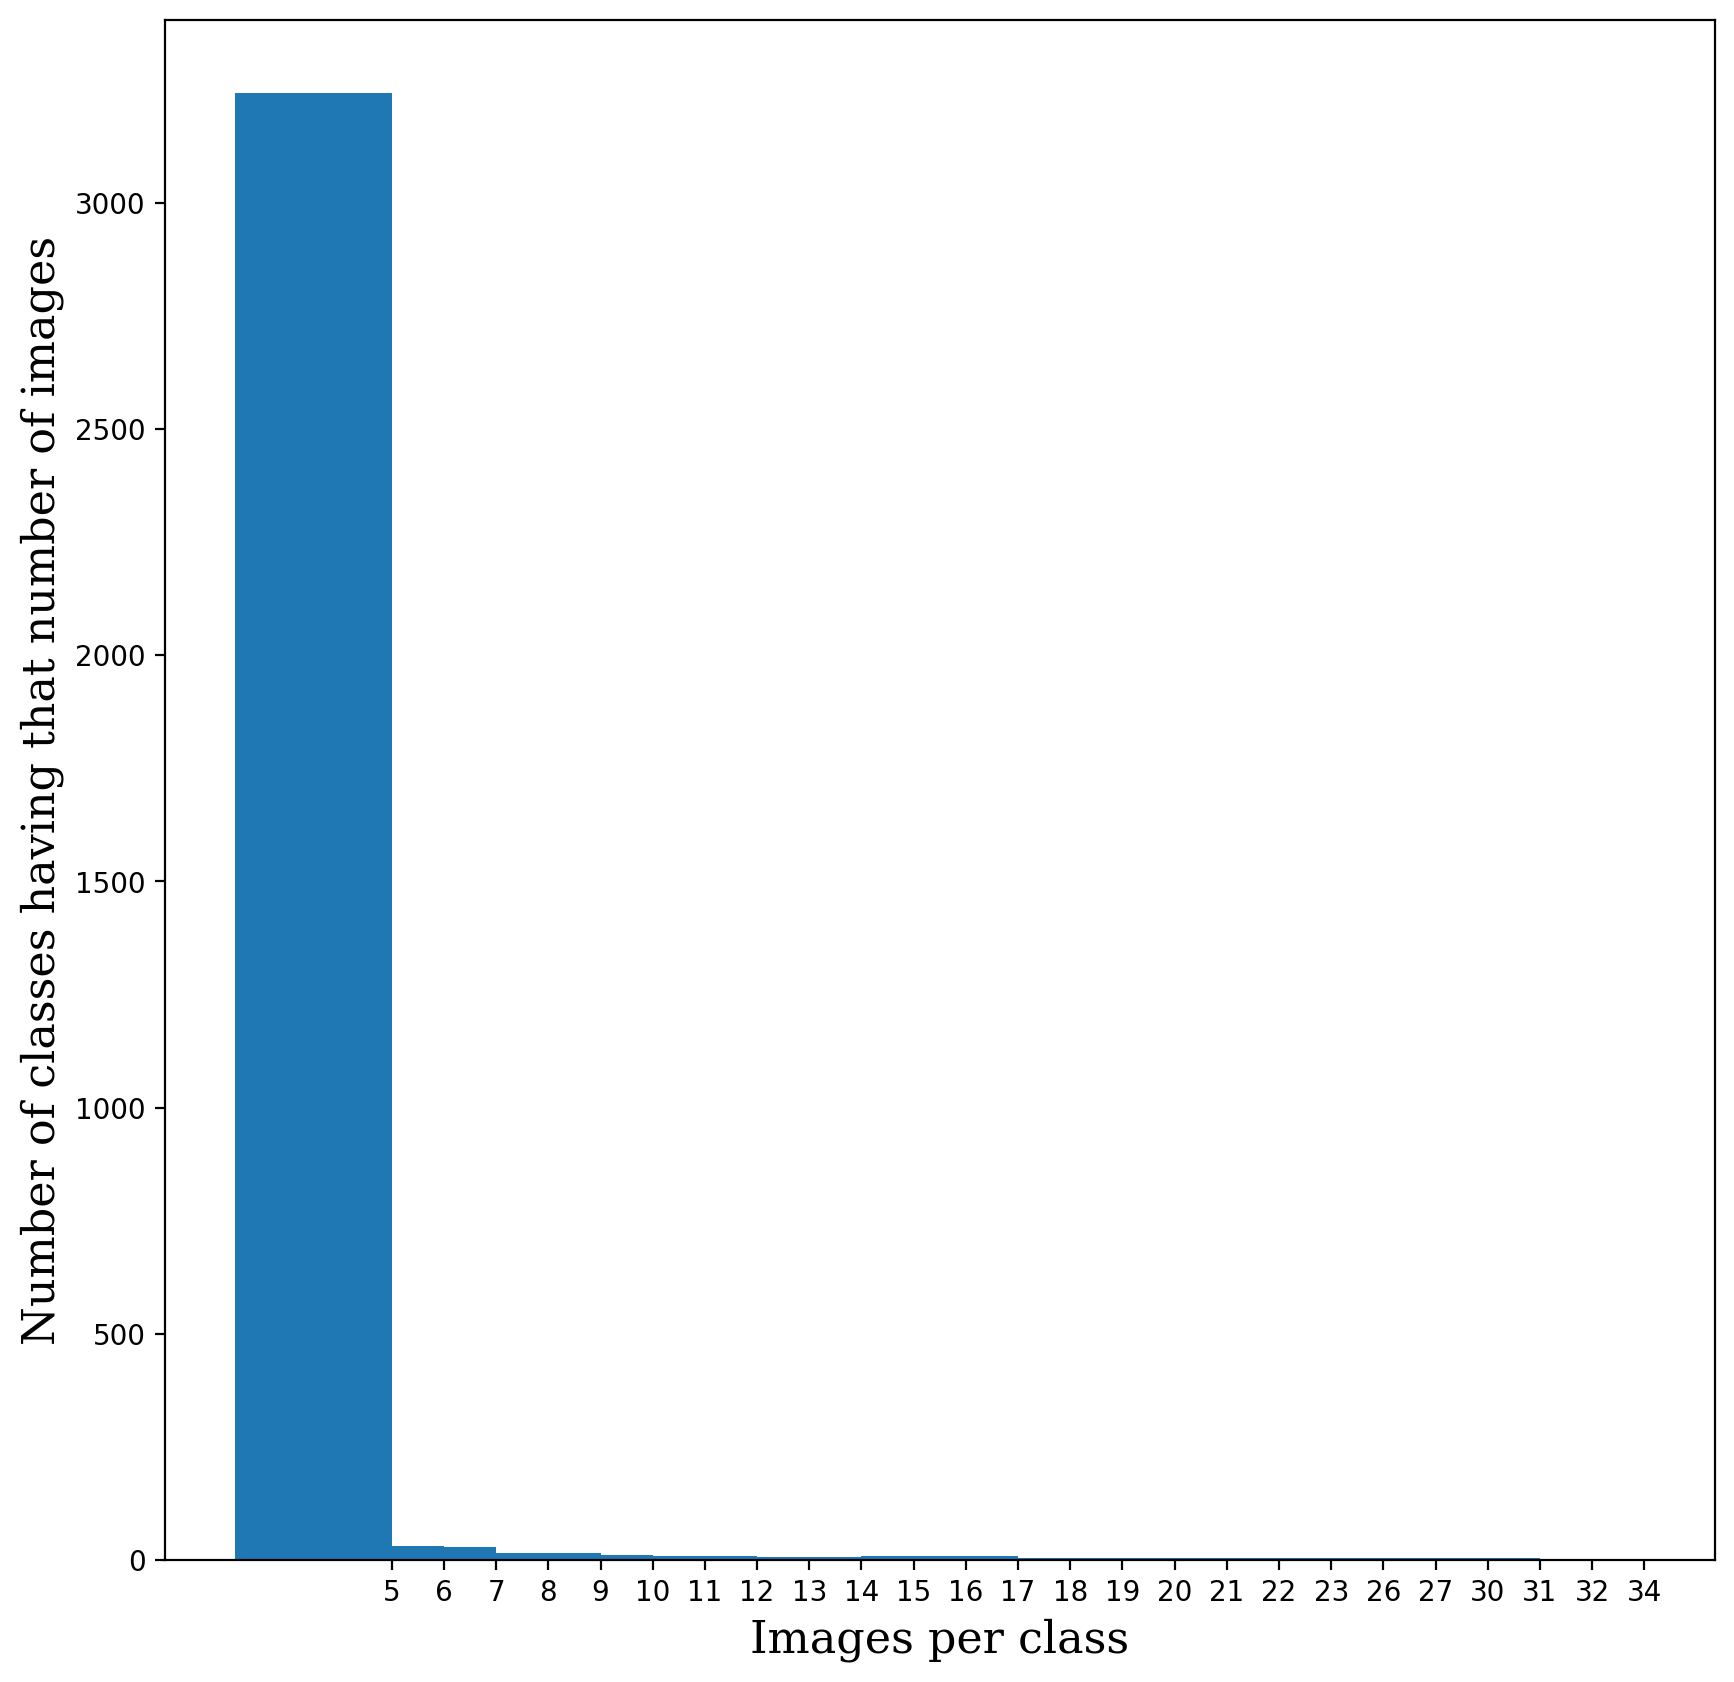
\includegraphics[width=.7\linewidth]{informatica/lfw_forzar_5}
        \caption{Forzando 5 imágenes por individuo}
    \end{subfigure}

    \begin{subfigure}{.5\textwidth}
        \centering
        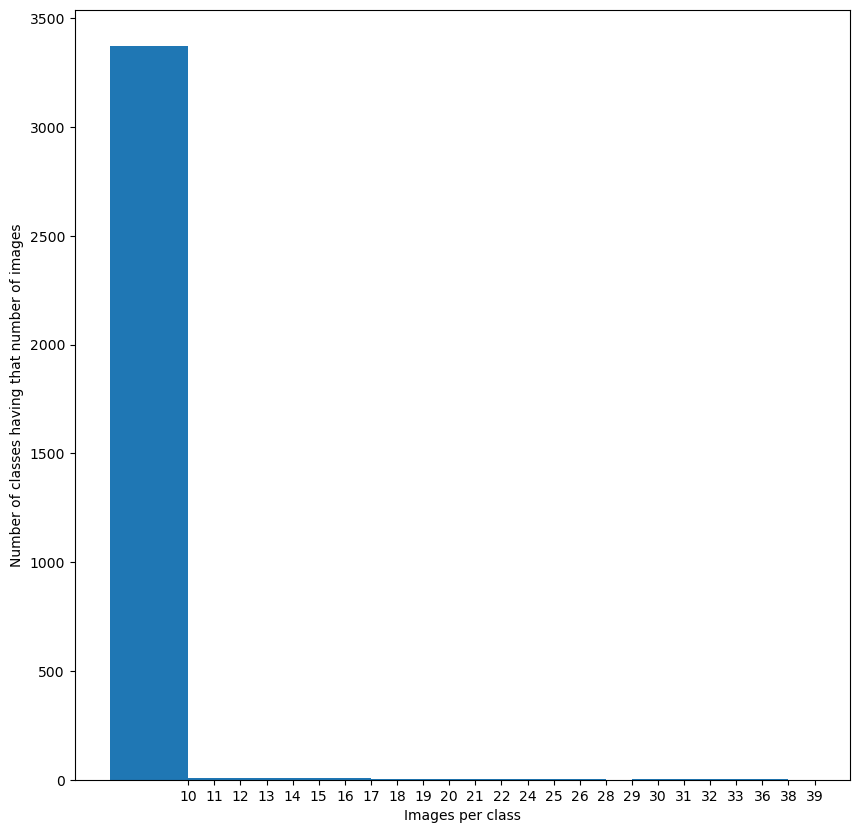
\includegraphics[width=.7\linewidth]{informatica/lfw_forzar_10}
        \caption{Forzando 10 imágenes por individuo }
    \end{subfigure}

    \caption{Distribuciones de imágenes por individuo tras aplicar \textit{dataset augmentation} para que cada clase tenga al menos $n$ individuos}
    \label{img:distribuciones_forzar_data_augmentation}
\end{figure}

Las distribuciones que se muestran en \customref{img:distribuciones_forzar_data_augmentation} muestran una propiedad clara: haciendo aumento de datos, la mayoría de individuos basan la variedad de sus imágenes en el aumento de datos. Además, esto ocurre por muy bajo que sea el número de imágenes por individuo que queramos obtener, como muestran las tres distribuciones prácticamente idénticas. Esto ya indica que seguramente los resultados obtenidos no sean demasiado buenos, puesto que la mayoría de imágenes de un individuo serán una o dos \entrecomillado{repetidas} (aunque apliquemos transformaciones propias del aumento de datos). Los posibles problemas que esto supone se agravan aún más al estar usando \textit{triplet loss} (\customref{isec:triplet_loss}).

Además, en este \textit{dataset} no tenemos información sobre las edades de los individuos en cada una de sus imágenes, así que no podemos hacer un estudio en más profundidad en este aspecto.

\subsection{\textit{FG-Net}} \label{isec:fgnet}
\todo{Ajustar el tamaño de las imágenes para que cuadren mejor los párrafos}

La \textbf{tercera base de datos} con la que trabajamos es \textit{FG-Net dataset}. La fuente original de este conjunto de datos ya no está operativa, y ahora estos datos se ofrecen en \cite{informatica:fgnet_dataset}. Este conjunto de datos se compone de 1002 imágenes de 82 individuos distintos. Es el \textit{dataset} más popular sobre \textit{AIFR} \cite{informatica:best_fgnet_model}.

\begin{figure}[H]
    \centering
    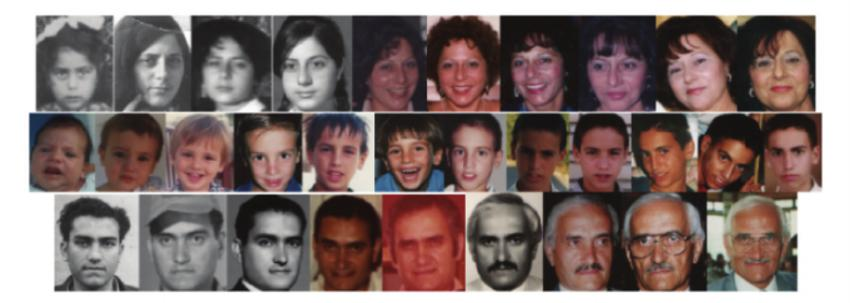
\includegraphics[width=0.8\textwidth]{informatica/ejemplo_fgnet}
    \caption{Muestra de ejemplo del \textit{dataset} \textit{FG-Net}. Imagen extraída de \url{https://paperswithcode.com/dataset/fg-net}}
\end{figure}

Este conjunto de datos no se ofrece en ninguna librería conocida de \textit{machine learning}. Por tanto, y como indicamos en \customref{isec:datasets_customs}, realizamos una implementación de \lstinline{torch.utils.data.Dataset} propia, para poder trabajar con estos datos.

Dicho conjunto de datos se compone de:

\begin{itemize}
    \item Un conjunto de imágenes. Los nombres de las imágenes deben ser procesados para extraer la identidad y edad de cada individuo
    \item Anotaciones de las imágenes. Estas anotaciones se componen de 68 puntos anotados por cada imagen
    \item Un archivo de \textit{Matlab} con 10 \textit{folds}, que el autor usa en \cite{informatica:yanweifu_work}
\end{itemize}

Optamos por trabajar únicamente con las imágenes, puesto que por las técnicas que estamos usando, no sabríamos aprovechar las anotaciones realizadas sobre los datos. Otros trabajos conocidos como \cite{informatica:facenet} usan esta forma de proceder. Gracias a los nombres de los archivos podemos almacenar también información sobre las edades de los individuos, información que nos va a ser muy relevante.

Y de nuevo, este \textit{dataset} presenta un salto de calidad respecto al anterior, por los siguientes motivos:

\begin{itemize}
    \item Trabajamos con un conjunto de datos cuya dificultad principal es la de la varianza en la edad. Esto se alinea por completo con el problema que queremos resolver
    \item El número de imágenes por individuo es mucho mejor que en \textit{LFW}, como muestran \customref{img:fgnet_images_per_class} y \customref{table:fgnet_images_per_class}
    \item Tenemos información sobre la distribución de la edad de nuestros individuos, que estudiamos en \customref{isubsubs:fgnet_dist_edades} y en \customref{isubsubs:fgnet_rango_edades}
\end{itemize}

\subsubsection{Distribución del número de imágenes por individuo}

A continuación, mostramos algunas características fundamentales del \textit{dataset}, empezando por la \textbf{distribución de número de imágenes por individuo}:

\begin{figure}[H]
    \centering
    \includegraphics[width=0.6\textwidth]{informatica/fgnet_images_per_class}
    \caption{Distribución del número de imágenes por cada individuo}
    \label{img:fgnet_images_per_class}
\end{figure}

Dicha distribución queda mejor explicada con las siguientes estadísticas:

\begin{table}[H]
\centering
\begin{tabular}{|l|l|}
    \hline
    \textbf{Estadística} & \textbf{Valor} \\
    \hline

    Media             & 12.22 \\
    Desviación típica & 2.15  \\
    Mínimo            & 6.00 \\
    Máximo            & 18.00 \\
    $Q1 \%$           & 11.00 \\
    $Q2 \%$           & 12.00 \\
    $Q3 \%$           & 13.00 \\

    \hline

\end{tabular}
\caption{Datos estadísticos sobre la distribución del número de imágenes por individuo}
\label{table:fgnet_images_per_class}
\end{table}

Tanto los estadísticos como la gráfica de la distribución dejan claro que, al menos en lo que respecta al número de imágenes por individuo, este conjunto de datos es mucho mejor. Como mínimo tenemos 6 imágenes por individuo, algo impensable en el conjunto de datos \textit{LFW}, donde apenas había individuos con más de dos imágenes. En segundo lugar, la media y los cuartiles nos muestran que la mayoría de los datos tienen entre 10 y 13 imágenes, lo que supone un muy buen dato.

\subsubsection{Distribución de edad de los individuos} \label{isubsubs:fgnet_dist_edades}

Veamos ahora la \textbf{distribución de la edad de los individuos}:

\begin{figure}[H]
    \centering
    \includegraphics[width=0.8\textwidth]{informatica/fgnet_distribucion_edades}
    \caption{Histograma de la variable edad en nuestro \textit{dataset}}
    \label{img:fgnet_histograma_edad}
\end{figure}

Que complementamos con las siguientes estadísticas

\begin{table}[H]
\centering
\begin{tabular}{|l|l|}
    \hline
    \textbf{Estadística} & \textbf{Valor} \\
    \hline

    Media  & 15.84 \\
    Mínimo & 0 \\
    Máximo & 69 \\
    Moda   & 18 \\

    \hline

\end{tabular}

    \caption{Algunas estadísticas sobre la distribución de la edad en nuestro conjunto de datos}
    \label{table:fgnet_estadisticas_edad}
\end{table}

El histograma \customref{img:fgnet_histograma_edad} nos muestra una distribución asímetrica, con una mayor concentración de individuos en edades bajas. Esto puede ser un problema a la hora de generalizar un modelo entrenado sobre estos datos, en el caso de que por ejemplo trabajemos con personas de una edad más adulta. Observando el histograma se observa un pico de frecuencia entorno a los 20 años. La moda nos indica que dicho pico se produce, en efecto, en los 18 años. Parece ser que dicha edad es un momento especial en el que se registran más fotografías de lo usual.

El rango de edades es muy amplio, yendo desde los 0 años (en \textit{LFW} ya comentábamos el problema que suponía no tener imágenes de niños) hasta los 69 años.

Por tanto, la calidad, en lo que distribución de edades se refiere, parece excelente. Aún así, podemos estudiar una distribución que nos dará una información todavía más profunda: el rango de edad por individuo.

\subsubsection{Distribución del rango de edad por individuo} \label{isubsubs:fgnet_rango_edades}

Estudiamos ahora el \textbf{rango de edad por individuo}. Para calcular este, computamos para cada individuo la diferencia entre su edad más avanzada menos su edad más temprana. Veamos este rango de edad gráficamente para todos los individuos:

\begin{figure}[H]
    \centering
    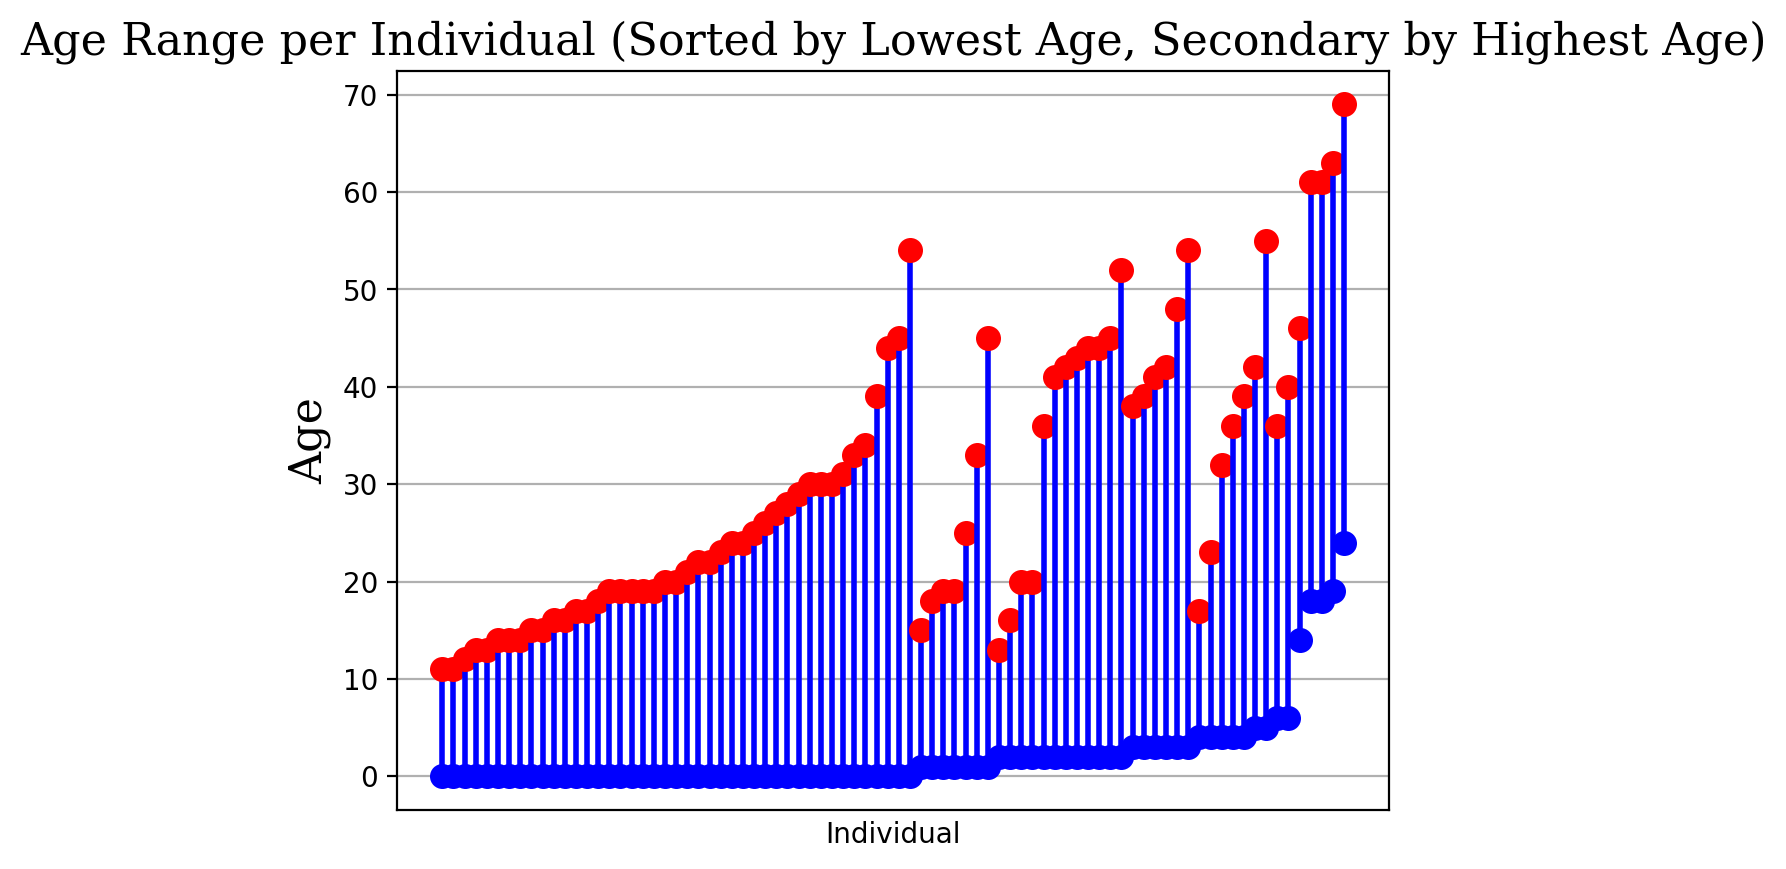
\includegraphics[width=0.8\textwidth]{informatica/fgnet_rangos_edad_individuales}
    \caption{Rangos de edad para todos los individuos. Los individuos están ordenados en primera instancia por su edad más baja, y en segunda instancia, por su edad más alta.}
    \label{img:fgnet_rangos_individuales}
\end{figure}

De esta forma es complicado sacar información de los datos. Así que mostremos la distribución de los rangos de edad:

\begin{figure}[H]
    \centering
    \includegraphics[width=0.8\textwidth]{informatica/fgnet_distribucion_rangos_edad}
    \caption{Distribución del rango de edad. En el eje horizontal tenemos los rangos de edad. En el eje vertical, la cantidad de individuos que presentan dicho rango de edad en sus imágenes}
    \label{img:fgnet_rangos_distribucion}
\end{figure}

Esta distribución se complementa con los siguientes datos estadísticos:

\begin{table}[H]
\centering
\begin{tabular}{|l|l|}
    \hline
    \textbf{Estadística} & \textbf{Valor} \\
    \hline

    Media             & 27.80 \\
    Desviación Típica & 11.75 \\
    Mínimo            & 11.00 \\
    $Q_1 \%$          & 18.00 \\
    $Q_2 \%$          & 26.50 \\
    $Q_3 \%$          & 37.75 \\
    Máximo            & 55.00 \\

    \hline

\end{tabular}
\caption{Datos estadísticos sobre la distribución de los rangos de edad}
\label{table:fgnet_rangos_estadisticas}
\end{table}

En base a estos datos, podemos observar:

\begin{itemize}
    \item El rango mínimo de edad es de 11 años. Esto es, dado cualquier individuo del conjunto de datos, tenemos aseguradas imágenes que difieren en al menos 11 años. El máximo rango es de 55 años. Esto supone una gran riqueza en los datos, y a la vez, una gran dificultad a la hora de trabajar la invarianza a los cambios de edad
    \item De media tenemos un rango de aproximadamente 27 años. Y la mayoría de nuestros datos se encuentran dentro de unas diferencias de edad de entre 18 y 37 años (aproximadamente). De nuevo, esto marca la calidad en cuanto a rangos de edad se refiere
    \item En \customref{img:fgnet_rangos_individuales} podemos ver claramente que la mayoría de individuos tienen imágenes en rangos de edad que podemos considerar bajos (por debajo de 10 años)
\end{itemize}

\subsubsection{Inconvenientes} \label{isubsubs:fgnet_inconvenientes}

Sin embargo, se presentan los siguientes \textbf{inconvenientes}:

\begin{enumerate}
    \item Partimos de trabajar con únicamente 1002 imágenes. Aunque lo hemos intentado, esta cantidad de datos no nos es suficiente para entrenar un modelo lo suficientemente potente de reconocimiento facial. Y mucho menos es suficiente para entrenar y además validar
    \item Como se comenta en \cite{informatica:best_fgnet_model}, este es el \textit{dataset} más famoso, pero a la vez, más complicado de resolver, en el ámbito de \textit{AIFR}. Esta complejidad ha quedado de sobra explicada en esta sección a través del estudio realizado, principalmente, sobre la distribución de edad y de rangos de edad
    \item Una forma de proceder común \cite{informatica:best_fgnet_model} es entrenar un modelo sobre un conjunto de datos mucho mayor, y usar este conjunto de datos únicamente para validar el modelo entrenado. Esta aproximación nos parece muy correcta por los siguientes motivos:
        \begin{itemize}
            \item En primer lugar, siempre es una buena idea comprobar que nuestro modelo generaliza correctamente, no solo sobre un subconjunto de datos de nuestro conjunto de trabajo original, sino sobre un conjunto de datos completamente nuevo
            \item En segundo lugar, hemos visto que la calidad de los datos en cuanto a rangos de edad es excelente, y supone un reto complejo. Por tanto, si obtenemos un modelo entrenado sobre otro conjunto de datos, que consigue un buen rendimiento en este, podemos estar bastante seguros de que nuestro modelo generalizará adecuadamente
            \item En tercer lugar, este proceso se asemeja bastante al uso que se le dará al modelo en la práctica, recibiendo imágenes de identidades nunca vistas con particularidades en el rango de edad que desconocemos a priori
        \end{itemize}
\end{enumerate}

Es por tanto que, siguiendo el procedimiento propuesto en \cite{informatica:best_fgnet_model}, usaremos este \textit{dataset} para validar el modelo entrenado sobre un conjunto de datos mucho mayor, en este caso, \customref{isec:dataset_cacd}.

\subsection{\textit{CACD}} \label{isec:dataset_cacd}

La \textbf{cuarta y última base de datos} con la que trabajamos es \entrecomillado{Cross-Age Celebrity Dataset} o \textit{CACD}. Como su propio nombre sugiere, se trata de una base de datos de celebridades en distintos momentos de su vida. Podemos acceder a estos datos en \cite{informatica:cacd_dataset}. El proceso de construcción de este conjunto de datos se especifica en \cite{informatica:paper_cacd}. En el momento de la publicación era el \textit{dataset} sobre \textit{AIFR} más grande.

Este \textit{dataset} se compone de 163446 imágenes de 2000 celebridades en edades que van desde los 16 hasta los 62 años \cite{informatica:paper_cacd}. Dichas imágenes fueron recolectadas de internet realizando búsquedas de ciertos individuos entre los años 2004 y 20013. Sabiendo la fecha de nacimiento de la celebridad, y el año de búsqueda, se computa la edad de dicha celebridad en cada imagen.

\begin{figure}[H]
    \centering
    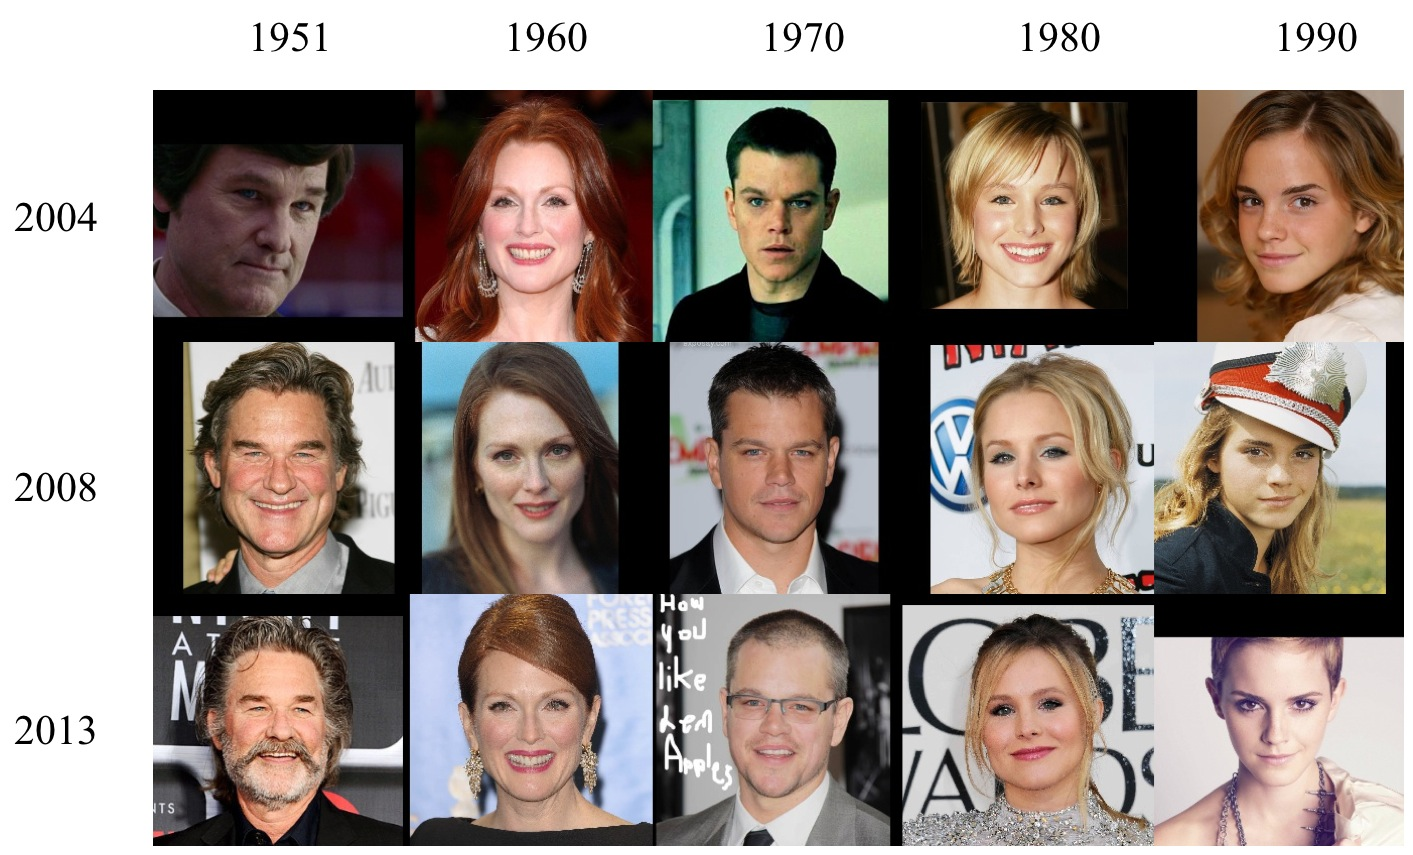
\includegraphics[width=0.8\textwidth]{informatica/cacd_example}
    \caption{Muestra de ejemplo del \textit{dataset} \textit{CACD}, imagen extraída de \cite{informatica:paper_cacd}. En la parte superior, tenemos anotadas los años de nacimiento de los individuos. En la parte izquierda, tenemos anotados los años en los que las imágenes fueron tomadas}
    \label{img:cacd_imagenes_ejemplo}
\end{figure}

De nuevo, este conjunto de datos no se ofrece en ninguna librería conocida de \textit{machine learning}, por lo que realizamos otra implementación de \lstinline{torch.utils.data.Dataset}, como desarrollamos en \customref{isec:datasets_customs}. El conjunto de datos se compone de:

\begin{itemize}
    \item Las imágenes de las celebridades
    \item Información sobre las celebridades: nombre, identificador en la base de datos, año de nacimiento, posicionamiento en la página \url{IMBD.com}, y si la celebridad aparece o no en el \textit{dataset} \textit{LFW}
    \item Información sobre cada imagen: identificador de la celebridad, edad de la celebridad en la imagen, año en el que se tomó la imagen y \textit{landmarks} faciales
\end{itemize}

De nuevo, trabajamos únicamente con el conjunto de datos de imágenes, sin anotaciones (como se hace, por ejemplo, en \cite{informatica:facenet}). De los propios nombres de los archivos podemos extraer el identificador de la celebridad y la edad que tiene en cada una de sus imágenes. Este conjunto de datos mantiene algunas de las características que deseábamos y trae otras nuevas:

\begin{itemize}
    \item En primer lugar, tenemos varianza en la edad de los individuos, que es fundamental para resolver nuestro problema
    \item El tamaño del conjunto de datos ahora es elevado, con lo que podemos plantearnos el aprendizaje de un modelo lo suficientemente potente
    \item El número de imágenes por individuo es excelente, aún mejor que en \textit{FG-Net}, como mostraremos en \customref{isubsubs:cacd_images_per_indv}
\end{itemize}

Además, como hemos comentado en \customref{isubsubs:fgnet_inconvenientes}, usaremos este \textit{dataset} en conjunto con \textit{FG-Net}. Sobre este conjunto de datos se realizará principalmente el entrenamiento, usando \textit{FG-Net} únicamente para validar el modelo obtenido.

Como hacíamos en \customref{isec:fgnet}, realizaremos un pequeño estudio de este conjunto de datos.

\subsubsection{Distribución del número de imágenes por individuo} \label{isubsubs:cacd_images_per_indv}

Veamos la \textbf{distribución del número de imágenes por cada individuo}:

\begin{figure}[H]
    \centering
    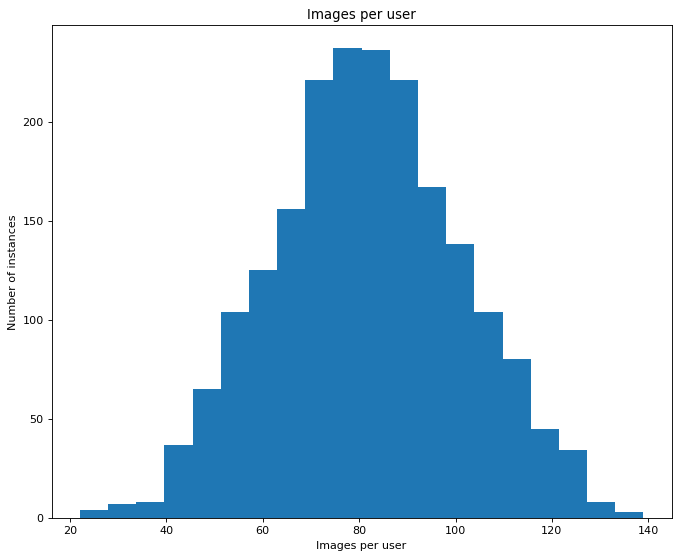
\includegraphics[width=0.6\textwidth]{informatica/cacd_images_per_class}
    \caption{Distribución del número de imágenes por cada individuo}
    \label{img:cacd_distr_images_per_class}
\end{figure}

De nuevo, complementamos con las siguientes estadísticas de la distribución:

\begin{table}[H]
\centering
\begin{tabular}{|l|l|}
    \hline
    \textbf{Estadística} & \textbf{Valor} \\
    \hline

    Media             & 81.72  \\
    Desviación típica & 19.51  \\
    Mínimo            & 22.00  \\
    $Q_1 \%$          & 68.00  \\
    $Q_2 \%$          & 81.00  \\
    $Q_3 \%$          & 95.00  \\
    Máximo            & 139.00 \\
    \hline

\end{tabular}
\caption{Datos estadísticos sobre la distribución del número de imágenes por individuo}
\end{table}

Podemos ver en \customref{img:cacd_distr_images_per_class}, que la distribución de imágenes por cada individuo parece seguir una distribución normal. Sin embargo, no nos interesa comprobar dicha hipótesis, pues es un hecho del que no vamos a aprovecharnos. Como mínimo, cada celebridad tiene 22 imágenes asociadas. Esto supone todavía una mejora respecto a \textit{FG-Net}. Llegamos a tener 139 imágenes por individuo como máximo. La mayoría de individuos tienen entre 68 y 95 imágenes asociadas. Por tanto, a la hora de establecer los valores del \textit{P-K sampling}, podemos tomar valores relativamente altos de $K$ (consultar \customref{ich:fundamentos_teoricos}).

\subsubsection{Distribución de edad de los individuos}

Veamos ahora la \textbf{distribución de edad de los individuos}:

\begin{figure}[H]
    \centering
    \includegraphics[width=0.6\textwidth]{informatica/cacd_distribucion_edades}
    \caption{Histograma de la variable edad en nuestro \textit{dataset}}
\end{figure}

Complementamos con las siguientes estadísticas:

\begin{table}[H]
\centering
\begin{tabular}{|l|l|}
    \hline
    \textbf{Estadística} & \textbf{Valor} \\
    \hline

    Media  & 38.03 \\
    Mínimo & 14    \\
    Máximo & 62    \\
    Moda   & 37    \\

    \hline

\end{tabular}
\caption{Algunas estadísticas sobre la distribución de la edad en nuestro conjunto de datos}
\end{table}

Esta vez tenemos una distribución más simétrica de las edades, con una media de aproximadamente 38 años. Las edad mínima es de 14 años, muy alejada de los 0 años de \textit{FG-Net} (\customref{table:fgnet_estadisticas_edad}). Esto puede suponer algunos problemas a la hora de entrenar un modelo en \textit{CACD} y que generalice correctamente en \textit{FG-Net}. No entraremos en comparaciones más profundas, pues esto lo haremos en \customref{isec:comparaciones_datasets}.

\subsubsection{Distribución del rango de edad por individuo}

Veamos ahora los \textbf{rangos de edad} de cada uno de los individuos del conjunto de datos:

\begin{figure}[H]
    \centering
    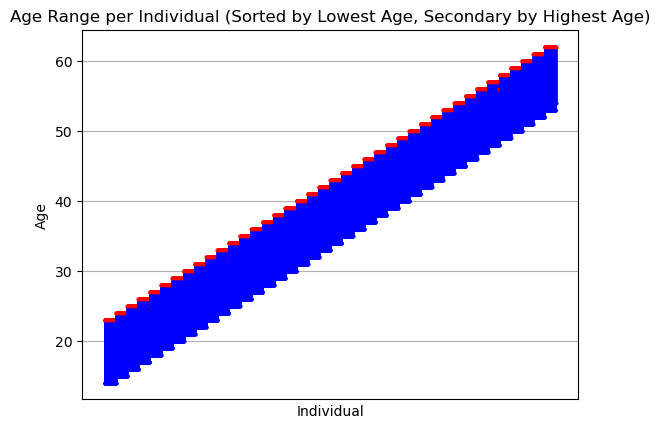
\includegraphics[width=0.6\textwidth]{informatica/cacd_rangos_individuales}
    \caption{Rangos de edad para todos los individuos. Los individuos están ordenados en primera instancia por su edad más baja, y en segunda instancia, por su edad más alta.}
\end{figure}

Esta gráfica ahora no es tan clara como cuando la presentábamos para \textit{FG-Net} en \customref{img:fgnet_rangos_distribucion}, así que procedemos a hacer unas observaciones. En primer lugar, como se han recolectado los datos buscando imágenes correspondientes al periodo 2004-2013, el rango de edad siempre va a ser de 9 años. Esto lo vamos a comprobar posteriormente. Por esto mismo, y por el ordenamiento en base a la edad más baja de cada individuo, estamos visualizando la distribución de las edades. Es decir, fijándonos en el punto más bajo de cada línea, estamos viendo a aquellos individuos que en 2004 tenían cierta edad. Así que se pueden visualizar, de una forma poco conveniente, los grupos de edad presentes en nuestra base de datos.

Confirmemos esto viendo las estadísticas sobre la distribución de los rangos de edad:

\begin{table}[H]
\centering
\begin{tabular}{|l|l|l|l|}
    \hline
    \textbf{Estadística} & \textbf{Valor} \\
    \hline

    Media             & 8.99 \\
    Desviación típica & 0.11 \\
    Mínimo            & 7.00 \\
    $Q_1 \%$          & 9.00 \\
    $Q_2 \%$          & 9.00 \\
    $Q_3 \%$          & 9.00 \\
    Máximo            & 9.00 \\

    \hline

\end{tabular}
    \caption{Datos estadísticos sobre la distribución de los rangos de edad}
\end{table}

Vemos que prácticamente todos los individuos tienen un rango de edad de nueve años. Podemos ver que tenemos un valor mínimo de 7 años. Por tanto, sabemos que tenemos algunos casos de individuos que no tienen cierta banda inicial o final de edades. Esto puede deberse a defunciones antes del 2013, o que el individuo era muy joven y no se disponían de imágenes suyas alrededor de 2004. Realizando una simple consulta sobre la base de datos, vemos que únicamente 15 individuos, de los 2000 individuos que componen la base de datos, tienen un rango de edad distinto a 9 años. Esto hace que sea completamente insignificativo.

Por tanto es totalmente innecesario mostrar el histograma de los rangos de edad.

\subsubsection{Inconvenientes}

Todo esto muestra los siguientes \textbf{inconvenientes}:

\begin{itemize}
    \item En primer lugar, los rangos de edad son muy pequeños y nada variables. Por ejemplo, viendo \customref{img:cacd_imagenes_ejemplo} las dos personas asociadas a las dos últimas columnas, podemos observar que hay poca variabilidad por el paso de los años. Además, nuestro modelo siempre va a trabajar con diferencias de como mucho 9 años, no sabemos cómo puede comportarse cuando presentemos imágenes con mayor diferencia en años
    \item En segundo lugar, y como comentaremos detalladamente en \label{isec:comparaciones_datasets}, el conjunto de entrenamiento y de validación son muy distintos (por ejemplo, no tenemos imágenes de personas por debajo de 14 años), y por tanto es realmente complicado que el modelo generalice. Sin embargo, de ser así, estaremos bastante seguros de haber construido un modelo robusto
\end{itemize}

\subsection{Comparación de los \textit{datasets} \textit{FG-Net} y \textit{CACD}} \label{isec:comparaciones_datasets}

Como hemos comentado, tanto en \customref{isec:fgnet} como en \customref{isec:dataset_cacd}, usaremos el segundo \textit{dataset} para entrenar nuestro modelo, y el segundo para validar los resultados obtenidos. Por tanto, es relevante realizar una comparación de ciertas propiedades de ambos conjuntos de datos. Repasaremos los apartados de estudio realizados en los dos últimos \textit{datasets}, comparando los resultados de ambos.


\subsubsection{Distribución del número de imágenes por individuo}

\begin{figure}[H]
\centering
    \begin{subfigure}{.5\textwidth}
        \centering
        \includegraphics[width=0.9\linewidth]{informatica/fgnet_images_per_class}
        \caption{\textit{FG-Net}}
    \end{subfigure}%
    \begin{subfigure}{.5\textwidth}
        \centering
        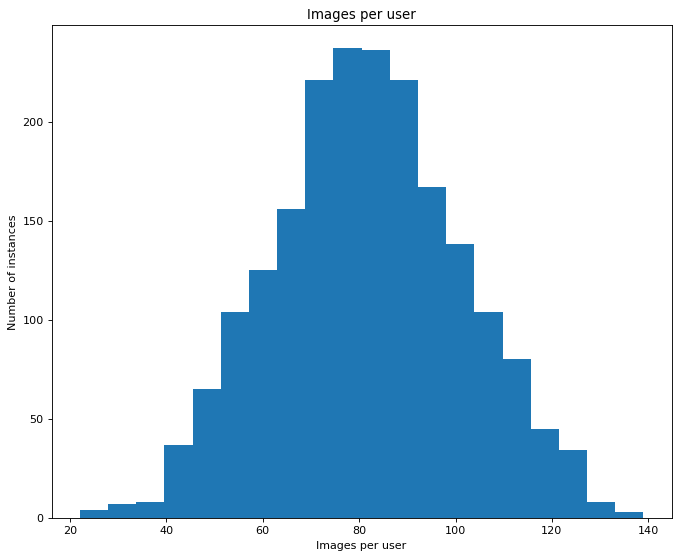
\includegraphics[width=0.9\linewidth]{informatica/cacd_images_per_class}
        \caption{\textit{CACD}}
    \end{subfigure}
\caption{Distribución del número de imágenes por individuo en los \textit{datsets} \textit{FG-Net} y \textit{CACD} }
\end{figure}


\begin{table}[H]
\centering
\begin{tabular}{|l|l|l|}
    \hline
    \textbf{\textit{Estadística}} & \textbf{\textit{FG-Net}} & \textbf{\textit{CACD}} \\
    \hline

    Media             & 12.22 & 81.72  \\
    Desviación típica & 2.15  & 19.51  \\
    Mínimo            & 6.00  & 22.00  \\
    Máximo            & 18.00 & 68.00  \\
    $Q1 \%$           & 11.00 & 81.00  \\
    $Q2 \%$           & 12.00 & 95.00  \\
    $Q3 \%$           & 13.00 & 139.00 \\

    \hline

\end{tabular}
\caption{Datos estadísticos sobre la distribución del número de imágenes por individuo, en los \textit{datasets} \textit{FG-Net} y \textit{CACD}}
\end{table}

Podemos ver, a partir de los datos, que:

\begin{itemize}
    \item El número de imágenes por individuo es ampliamente superior en \textit{CACD} que en \textit{FG-Net}. Un claro indicador de esto es que el valor máximo en \textit{FG-Net} está por debajo del máximo en \textit{CACD}. Este hecho puede ayudar a solventar algunos de los problemas sobre la diferencia en la distribución de la edad que plantea \textit{FG-Net}
    \item La desviación típica es mucho menor en \textit{FG-Net}. Por lo tanto, en cuanto a cuántas imágenes podemos encontrar por cada individuo, quizás \textit{CACD} introduzca algo más de dificultad, aunque esto no nos parece un factor realmente relevante
    \item A la hora de entrenar, vamos a poder usar valores mucho más altos de $K$ en \textit{CACD} (véase \customref{ich:fundamentos_teoricos} para más detalles). Y este valor, en validación, se puede reducir (o directamente ignorar) para actuar sobre \textit{FG-Net}
    \item La distribución en \textit{CACD} parece seguir una distribución normal, mientras que en \textit{FG-Net}, a priori, no se ve de forma tan clara. Aunque como ya hemos comentado previamente, no estamos interesados en comprobar estas hipótesis
\end{itemize}

\subsubsection{Distribución de edad de los individuos} \label{isubsubs:conjunta_fgnet_cacd_edades}

\begin{figure}[H]
\centering
    \begin{subfigure}{.5\textwidth}
        \centering
        \includegraphics[width=0.9\linewidth]{informatica/fgnet_distribucion_edades}
        \caption{\textit{FG-Net}}
    \end{subfigure}%
    \begin{subfigure}{.5\textwidth}
        \centering
        \includegraphics[width=0.9\linewidth]{informatica/cacd_distribucion_edades}
        \caption{\textit{CACD}}
    \end{subfigure}
    \caption{Distribuciones de las edades en los \textit{datasets} \textit{FG-Net} y \textit{CACD}}
    \label{img:conjunta_fgnet_cacd_edades}
\end{figure}

\begin{table}[H]
\centering
\begin{tabular}{|l|l|l|}
    \hline
    \textbf{Estadística} & \textbf{\textit{FG-Net}} & \textbf{\textit{CACD}} \\
    \hline

    Media  & 15.84 & 38.03 \\
    Mínimo & 0     & 14    \\
    Máximo & 69    & 62    \\
    Moda   & 18    & 37    \\

    \hline

\end{tabular}
    \caption{Estadísticas sobre la distribución de la edad en los \textit{datasets} \textit{FG-Net} y \textit{CACD}}
    \label{table:conjunta_fgnet_cacd_estadisticas_edad}
\end{table}

A partir de estos datos, podemos ver que:

\begin{itemize}
    \item Las formas de las dos distribuciones de datos, tal y como se aprecia en \customref{img:conjunta_fgnet_cacd_edades}, son completamente distintas. Por un lado, en \textit{FG-Net} tenemos una distribución muy asimétrica, acumulando la mayor parte de la densidad en edades bajas, entre 0 y 20 años. En \textit{CACD}, tenemos una distribución más o menos simétrica
    \item El dominio en \textit{FG-Net} es mucho más amplio, con una edad mínima 14 años menor, y una edad máxima 7 años mayor
    \item Por tanto, era razonable pensar que íbamos a tener una población mucho más adulta en \textit{CACD}, como muestran tanto los histogramas como el valor de la media y moda en \customref{table:conjunta_fgnet_cacd_estadisticas_edad}
    \item La concentración en edades bajas en \textit{FG-Net} puede presentar un \textbf{serio problema} a la hora de que un modelo entrenado sobre \textit{CACD} funcione correctamente
\end{itemize}


\subsubsection{Distribución del rango de edad por individuo}

\begin{figure}
\centering
    \begin{subfigure}{.5\textwidth}
        \centering
        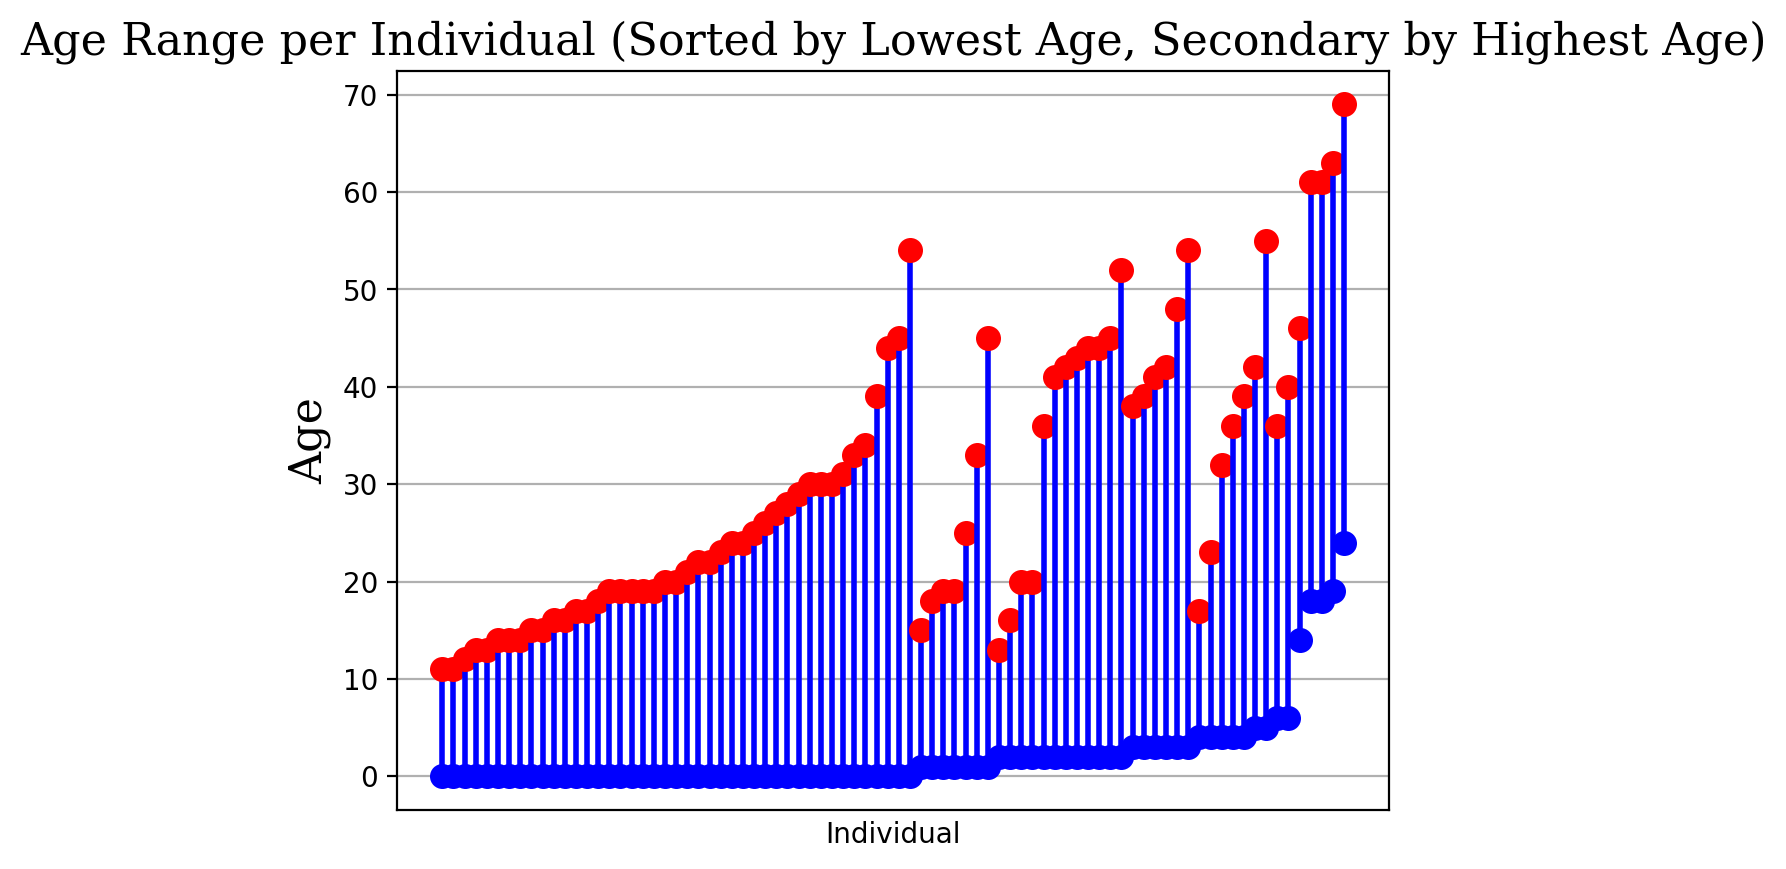
\includegraphics[width=0.9\linewidth]{informatica/fgnet_rangos_edad_individuales}
        \caption{\textit{FG-Net}}
    \end{subfigure}%
    \begin{subfigure}{.5\textwidth}
        \centering
        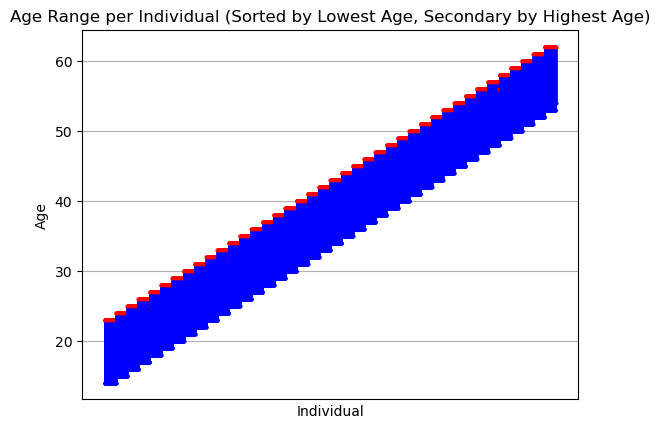
\includegraphics[width=0.9\linewidth]{informatica/cacd_rangos_individuales}
        \caption{\textit{CACD}}
    \end{subfigure}
\caption{Rangos de edad para todos los individuos, en los \textit{datasets} \textit{FG-Net} y \textit{CACD}. Los individuos están ordenados en primera instancia por su edad más baja, y en segunda instancia, por su edad más alta.}
\label{img:conjunta_fgnet_rangos_edades_individuales}
\end{figure}

\begin{table}[H]
\centering
\begin{tabular}{|l|l|l|}
    \hline
    \textbf{Estadística} & \textbf{\textit{FG-Net}} & \textbf{\textit{CACD}} \\
    \hline

    Media             & 27.80 & 8.99 \\
    Desviación Típica & 11.75 & 0.11 \\
    Mínimo            & 11.00 & 7.00 \\
    $Q_1 \%$          & 18.00 & 9.00 \\
    $Q_2 \%$          & 26.50 & 9.00 \\
    $Q_3 \%$          & 37.75 & 9.00 \\
    Máximo            & 55.00 & 9.00 \\

    \hline

\end{tabular}
\caption{Datos estadísticos sobre la distribución de los rangos de edad, para los \textit{datasets} \textit{FG-Net} y \textit{CACD}}
    \label{table:conjunta_fgnet_estadisticas_rangos_edad}
\end{table}

A partir de estos datos, podemos observar que:

\begin{itemize}
    \item Como muestran tanto \customref{img:conjunta_fgnet_rangos_edades_individuales} como \customref{table:conjunta_fgnet_estadisticas_rangos_edad}, \textit{FG-Net} presenta una variabilidad en los rangos de edad que es prácticamente inexistente en \textit{CACD} (en la que salvo 15 individuos, el rango de edad siempre es de 15 años)
    \item Este problema se ve agravado cuando nos damos cuenta que la mayoría de individuos en \textit{FG-Net} tienen un rango de edades entre 18 y casi 38 años, que contrasta con el rango de 9 años constante en \textit{CACD}. Si el rango en \textit{CACD} fuese constante pero superior, al menos la falta de variabilidad podría no notarse tanto
    \item Para \textit{FG-Net} tenía sentido mostrar el histograma de la distribución de rangos, en \customref{img:fgnet_rangos_distribucion}. Sin embargo, en \textit{CACD}, como no teníamos variabilidad, no mostramos dicho histograma
    \item Así que las dificultades que veíamos en \customref{isubsubs:conjunta_fgnet_cacd_edades} se ven agravadas al estudiar la distribución de los rangos de edad
\end{itemize}

\section{Descripción de los objetivos}
\todo{Esta sección no me convence nada, volver a ella cuando haya desarrollado más texto}

Por todo esto, los objetivos del presente trabajo son los siguientes:

\begin{enumerate}
    \item Realizar una revisión del estado del arte en el ámbito del \textit{AIFR}
    \item Implementar todos los módulos necesarios para poder aplicar técnicas \textit{online} de cómputo del \textit{triplet loss}
    \item Realizar un estudio de los \textit{datasets} disponibles
        \todo{No sé que sentido tiene hablar de esto aquí cuando acabamos de mirar todos los datasets que vamos a usar (aunque no todos los datasets disponibles)}
    \item Comparar los resultados obtenidos con otros trabajos del mismo ámbito
    \item Los \textit{scripts} con los que el autor genera las anotaciones de los datos
\end{enumerate}

\section{Planificación} \label{isec:planificacion}

Tras un estudio inicial de los \textit{frameworks} de aprendizaje automático existentes, nos damos cuenta de que no hay implementaciones para las técnicas que queremos explorar. Esto supone que \textbf{deberemos dedicar un gran esfuerzo al diseño, implementación, optimización y validación de módulos de código}. Por tanto, decidimos realizar un desarrollo en varias etapas, iterando sobre distintas bases de datos, de menor complejidad (estructura de los datos, facilidad de trabajo con ellos, tamaño) e interés, hasta los datos más complejos y relevantes para nuestro estudio. Como veremos en \customref{isec:optimizacion_codigo}, esto permite en un inicio desarrollar rápidamente una amplia base de código sin preocuparnos de realizar optimizaciones prematuras y poco relevantes. Solo se realiza un proceso de optimización cuando encontramos problemas reales con los tiempos de cómputo.

Una vez analizados y resuelto los puntos débiles en temas de rendimiento pasamos a tratar con las bases de datos que realmente nos interesan. Así, en este punto, tenemos prácticamente toda la base de código desarrollada, pudiendo centrarnos únicamente en la experimentación.

Las bases de datos sobre las que iteramos se describen con detalle en \customref{isec:base_datos_usada}.

Además, como veremos en \customref{ich:estado_arte}, \textbf{no existen trabajos previos que hayan aplicado nuestro enfoque para resolver el problema de \textit{AIFR}}. Por tanto, esperamos encontrarnos con dificultades desconocidas, tanto en la implementación como en la experimentación, que deberemos resolver sin tener literatura específica sobre la que apoyarnos.

Todo esto justifica que no escojamos un modelo de desarrollo en cascada clásico: no sabemos cuándo nos vamos a enfrentar con problemas de rendimiento y, por la falta de literatura sobre el tema, desconocemos los posibles problemas que pueden resultar de aplicar esta técnica. Por lo tanto, \textbf{decidimos usar un modelo de desarrollo iterativo} \cite{informatica:libro_metodologias_desarrollo}. En este modelo de desarrollo, realizamos varias iteraciones. En cada una de las iteraciones podemos aplicar el modelo en cascada. Este modelo encaja perfectamente con nuestro enfoque, en el que buscamos iterar sobre distintas bases de datos. El funcionamiento de este modelo se explica mejor en la siguiente imagen:

\begin{figure}[H]
    \centering
    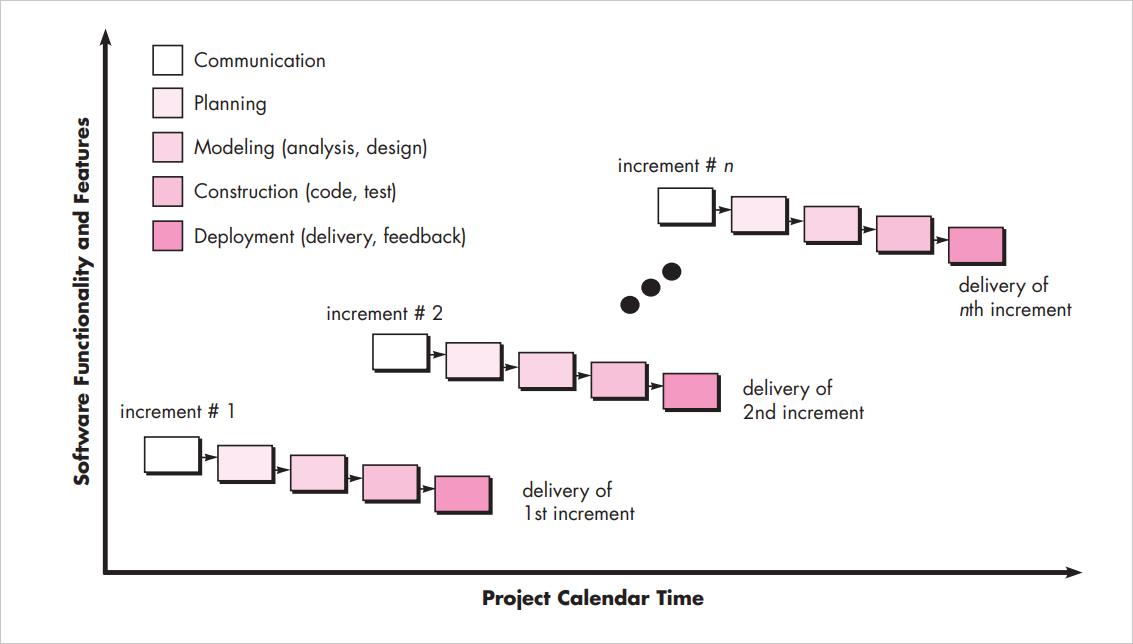
\includegraphics[width=0.8\textwidth]{informatica/ejemplo_modelo_incremental}
    \caption{Ejemplo del modelo de desarrollo incremental. Podemos ver que en cada iteración aplicamos un modelo de desarrollo en cascada. En nuestro caso, cada iteración corresponderá con cada una de las bases de datos sobre las que iteramos. Imagen extraída de \cite{informatica:libro_metodologias_desarrollo}}
\end{figure}

Para cada base de datos sobre la que trabajamos, consideramos las siguientes fases del modelo en cascada para esa iteración:

\begin{itemize}
    \item Análisis: realizamos un análisis exploratorio de la base de datos con la que trabajamos en esta iteración (véase \customref{isec:base_datos_usada}). Estudiamos las técnicas que queremos aplicar y nos marcamos una serie de objetivos para esta iteración
    \item Diseño: en base al estudio realizado sobre el \textit{dataset} y las técnicas que queremos aplicar, definimos qué módulos de código debemos de introducir, qué interfaces deben cumplir para interactuar con otros módulos de código, las propiedades que queremos verificar en los \textit{tests}, distintos \textit{pipelines} que seguir en la experimentación...
    \item Implementación: desarrollamos el código necesario para cumplir con el diseño realizado previamente. En esta fase también incluimos el desarrollo de \textit{tests} para realizar las validaciones
    \item Optimización: en esta fase realizamos \textit{profiles} para detectar partes críticas del código, introducimos \textit{benchmarks} para estudiar el impacto de los cambios realizados, y llevamos a cabo dichos cambios. Esto se explica en detalle en \customref{isec:optimizacion_codigo}. Esta fase es opcional, no se realiza salvo que en la iteración se detecten problemas de rendimiento relevantes
    \item Experimentación: lanzamos los \textit{pipelines} desarrollados en la fase anterior (véase \customref{isec:pipeline}), analizamos los resultados obtenidos, buscamos anomalías en el proceso o en los resultados, ... Esta fase es fundamental a la hora de marcar los objetivos y problemas a resolver en la siguiente iteración sobre una nueva base de datos
\end{itemize}

Para organizar todas las tareas de cada iteración, que nacen en las fases de análisis, diseño e implementación, usamos la \textbf{metodología \textit{Kanban}} \cite{informatica:kanban_paper}. En dicha metodología se usa un tablero, en el que tarjetas que representan tareas a realizar se colocan sobre columnas que representan distintos estados. Usamos cuatro estados:

\begin{itemize}
    \item \textit{Backlog} o tareas que no sabemos si vamos a llevar a cabo
    \item \textit{To-do} o tareas que debemos llevar a cabo.
    \item \textit{In-progress} o tareas que actualmente estamos trabajando
    \item \textit{Done} o tareas que ya se han completado
\end{itemize}

Esto permite tener una visualización rápida del estado de la iteración. Como comentaremos detalladamente en \customref{isec:github_buenas_practicas}, usaremos la utilidad de proyectos que ofrece \textit{Github} para tener acceso a un tablero \textit{kanban}. En la siguiente imagen se muestra un ejemplo del estado de este tablero:

\begin{figure}[H]
    \centering
    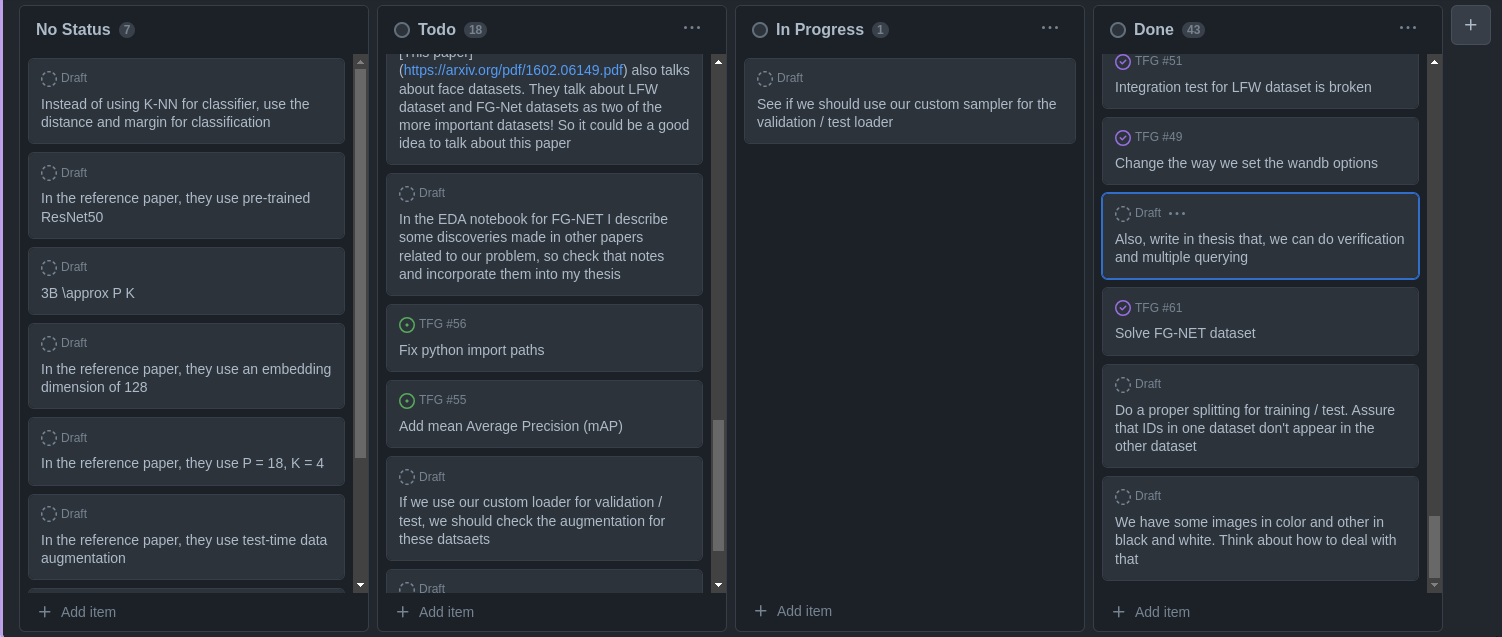
\includegraphics[width=0.9\textwidth]{informatica/kanban_board}
    \caption{Ejemplo del estado de nuestro tablero \textit{kanban} en un momento concreto durante la fase de desarrollo. Podemos ver las cuatro columnas que ya hemos descrito. \textit{Github} le da el nombre \textit{No Status} a la columna que nosotros usamos como \textit{backlog}}
\end{figure}

Comenzamos a desarrollar el proyecto en Febrero de 2022. Sabemos que, debido a los exámenes universitarios, apenas trabajaremos en los meses de Enero, Mayo y Junio. Por tanto, consideraremos que en estos meses no trabajemos ninguna hora (aunque en la práctica sí que consigamos sacar algo de tiempo). Los meses en los que más trabajaremos serán Febrero, Julio, Agosto y Septiembre. En estos meses tenemos previsto trabajar al menos 20 horas semanales. En el resto de meses consideramos que trabaremos al menos 2 horas semanales. Por tanto, en los dos años que dedicamos al proyecto de informática, dedicaremos al menos 720 horas.

Teniendo todo esto en cuenta, inicialmente planificamos el proyecto tal y como describe el siguiente diagrama de Gannt:

\begin{figure}[H]
    \centering
    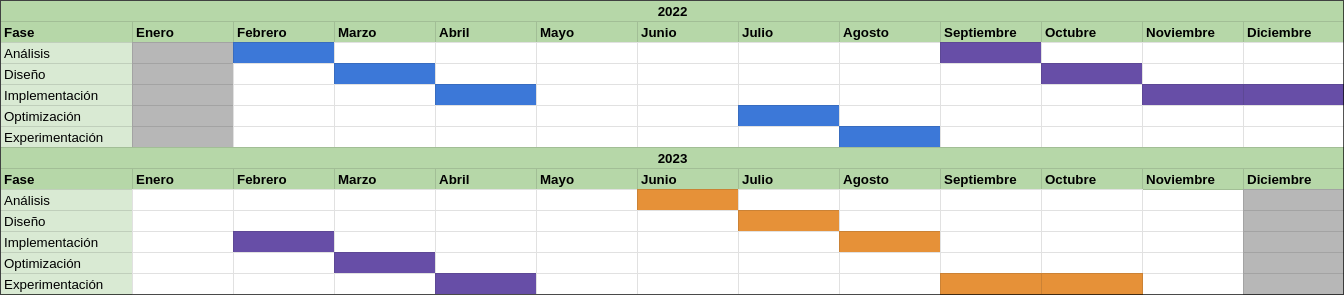
\includegraphics[width=1.0\textwidth]{informatica/diagrama_gannt_ideal}
    \caption{Diagrama de \textit{Gantt} que describe la planificación original del proyecto. El color azul corresponde al \textit{dataset} \textit{MNIST}. El color morado corresponde al \textit{dataset} \textit{LFW}. El color naranja corresponde a los \textit{datasets} \textit{FG-Net} junto con \textit{CACD}}
\end{figure}

Sin embargo, por los problemas enfrentados durante el desarrollo, y por inexactitudes en la planificación, acabamos distribuyendo el tiempo dedicado al trabajo tal y como se muestra en el siguiente diagrama de Gannt:

\begin{figure}[H]
    \centering
    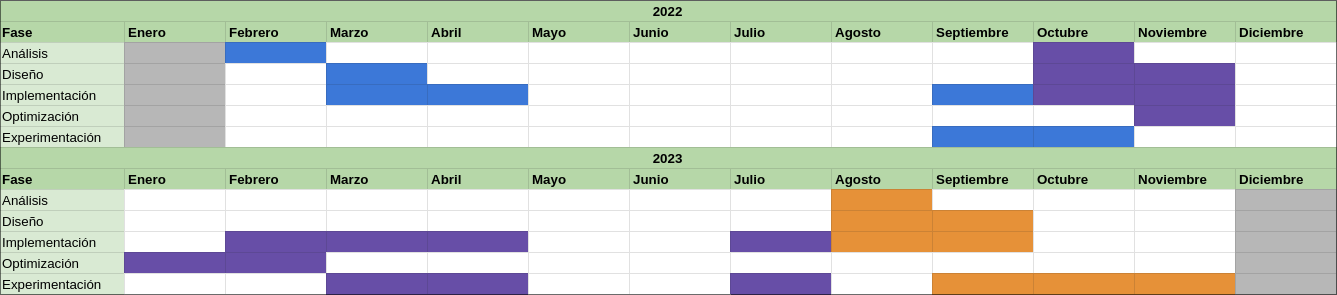
\includegraphics[width=1.0\textwidth]{informatica/diagrama_gannt_real}
    \caption{Diagrama de \textit{Gantt} que describe la distribución real del tiempo dedicado al proyecto. Seguimos el mismo código de colores que en el diagrama anterior}
    \label{img:gannt_real}
\end{figure}

En el repositorio abierto de \textit{Github} \cite{informatica:repogithub} donde hemos desarrollado el proyecto, podemos verificar los tiempos que aparecen en \customref{img:gannt_real}.

En cuanto a la planificación económica, tenemos en cuenta los siguientes aspectos:

\begin{itemize}
    \item El salario aproximado de un investigador en Ciencia de Datos y Aprendizaje Automático es de 35 €/h. Teniendo en cuenta que hemos dedicado al menos 720 horas de trabajo, esto supone un coste de 25.200€
    \item El valor del ordenador que hemos usado para trabajar: 600€
    \item El valor de los servidores \textit{nGPU} donde se han lanzado los procesos (véase \customref{isec:entorno_ejecucion}). Se estima un coste de unos 145€ semanales. Teniendo en cuenta que hemos tenido acceso desde Marzo de 2023, y usamos estos servidores hasta Octubre de 2023, esto supone un coste de 4.640€
\end{itemize}

Todo esto supone un \textbf{coste total} de unos 30.440€.
